% OLD
%\documentclass[11pt,compress,t,notes=noshow, aspectratio=169, xcolor=table]{beamer}
% new
\documentclass[10pt,compress,t,notes=noshow, xcolor=table]{beamer}

% OLD
%\usepackage{../../style/lmu-lecture}
% new
\usepackage[]{graphicx}
% graphicx is loaded via lmu-lecture.sty as well
\usepackage[]{color}
% maxwidth is the original width if it is less than linewidth
% otherwise use linewidth (to make sure the graphics do not exceed the margin)
\makeatletter
\def\maxwidth{ %
  \ifdim\Gin@nat@width>\linewidth
    \linewidth
  \else
    \Gin@nat@width
  \fi
}
\makeatother

% ---------------------------------%
% latex-math dependencies, do not remove:
% - mathtools
% - bm
% - siunitx
% - dsfont
% - xspace
% ---------------------------------%

%--------------------------------------------------------%
%       Language, encoding, typography
%--------------------------------------------------------%

\usepackage[english]{babel}
\usepackage[utf8]{inputenc} % Enables inputting UTF-8 symbols
% Standard AMS suite (loaded via lmu-lecture.sty)
\usepackage{amsmath,amsfonts,amssymb}

% Font for double-stroke / blackboard letters for sets of numbers (N, R, ...)
% Distribution name is "doublestroke"
% According to https://mirror.physik.tu-berlin.de/pub/CTAN/fonts/doublestroke/dsdoc.pdf
% the "bbm" package does a similar thing and may be superfluous.
% Required for latex-math
\usepackage{dsfont}

% bbm – "Blackboard-style" cm fonts (https://www.ctan.org/pkg/bbm)
% Used to be in common.tex, loaded directly after this file
% Maybe superfluous given dsfont is loaded
% TODO: Check if really unused?
% \usepackage{bbm}

% bm – Access bold symbols in maths mode - https://ctan.org/pkg/bm
% Required for latex-math, preferred over \boldsymbol
% https://tex.stackexchange.com/questions/3238/bm-package-versus-boldsymbol
\usepackage{bm}

% pifont – Access to PostScript standard Symbol and Dingbats fonts
% Used for \newcommand{\xmark}{\ding{55}, which is never used
% aside from lecture_advml/attic/xx-automl/slides.Rnw
% \usepackage{pifont}

% Quotes (inline and display), provdes \enquote
% https://ctan.org/pkg/csquotes
\usepackage{csquotes}

% Adds arg to enumerate env, technically superseded by enumitem according
% to https://ctan.org/pkg/enumerate
% Replace with https://ctan.org/pkg/enumitem ?
% Even better: enumitem is not really compatible with beamer and breaks all sorts of things
% particularly the enumerate environment. The enumerate package also just isn't required
% from what I can tell so... don't re-add it I guess?
% \usepackage{enumerate}

% Line spacing - provides \singlespacing \doublespacing \onehalfspacing
% https://ctan.org/pkg/setspace
% \usepackage{setspace}

% mathtools – Mathematical tools to use with amsmath
% https://ctan.org/pkg/mathtools?lang=en
% latex-math dependency according to latex-math repo
\usepackage{mathtools}

% Maybe not great to use this https://tex.stackexchange.com/a/197/19093
% Use align instead -- TODO: Global search & replace to check, eqnarray is used a lot
% $ rg -f -u "\begin{eqnarray" -l | grep -v attic | awk -F '/' '{print $1}' | sort | uniq -c
%   13 lecture_advml
%   14 lecture_i2ml
%    2 lecture_iml
%   27 lecture_optimization
%   45 lecture_sl
\usepackage{eqnarray}

% For shaded regions / boxes
% Used sometimes in optim
% https://www.ctan.org/pkg/framed
\usepackage{framed}

%--------------------------------------------------------%
%       Cite button (version 2024-05)
%--------------------------------------------------------%
% Note this requires biber to be in $PATH when running,
% telltale error in log would be e.g. Package biblatex Info: ... file 'authoryear.dbx' not found
% aside from obvious "biber: command not found" or similar.
% Tried moving this to lmu-lecture.sty but had issues I didn't quite understood,
% so it's here for now.

\usepackage{textcase} % for \NoCaseChange
\usepackage{hyperref}

% Only try adding a references file if it exists, otherwise
% this would compile error when references.bib is not found
\IfFileExists{references.bib} {
  \usepackage{usebib}
  \usepackage[backend=biber, style=authoryear]{biblatex}

  \addbibresource{./references.bib}
  \bibinput{references}
}

\newcommand{\citelink}[1]{%
\NoCaseChange{\resizebox{!}{9pt}{\protect\beamergotobutton{\href{\usebibentry{\NoCaseChange{#1}}{url}}{\begin{NoHyper}\cite{#1}\end{NoHyper}}}}}%
}

%--------------------------------------------------------%
%       Displaying code and algorithms
%--------------------------------------------------------%

% Reimplements verbatim environments: https://ctan.org/pkg/verbatim
% verbatim used sed at least once in
% supervised-classification/slides-classification-tasks.tex
% Removed since code should not be put on slides anyway
% \usepackage{verbatim}

% Both used together for algorithm typesetting, see also overleaf: https://www.overleaf.com/learn/latex/Algorithms
% algorithmic env is also used, but part of the bundle:
%   "algpseudocode is part of the algorithmicx bundle, it gives you an improved version of algorithmic besides providing some other features"
% According to https://tex.stackexchange.com/questions/229355/algorithm-algorithmic-algorithmicx-algorithm2e-algpseudocode-confused
\usepackage{algorithm}
\usepackage{algpseudocode}

%--------------------------------------------------------%
%       Tables
%--------------------------------------------------------%

% multi-row table cells: https://www.namsu.de/Extra/pakete/Multirow.html
% Provides \multirow
% Used e.g. in evaluation/slides-evaluation-measures-classification.tex
\usepackage{multirow}

% colortbl: https://ctan.org/pkg/colortbl
% "The package allows rows and columns to be coloured, and even individual cells." well.
% Provides \columncolor and \rowcolor
% \rowcolor is used multiple times, e.g. in knn/slides-knn.tex
\usepackage{colortbl}

% long/multi-page tables: https://texdoc.org/serve/longtable.pdf/0
% Not used in slides
% \usepackage{longtable}

% pretty table env: https://ctan.org/pkg/booktabs
% Is used
% Defines \toprule
\usepackage{booktabs}

%--------------------------------------------------------%
%       Figures: Creating, placing, verbing
%--------------------------------------------------------%

% wrapfig - Wrapping text around figures https://de.overleaf.com/learn/latex/Wrapping_text_around_figures
% Provides wrapfigure environment -used in lecture_optimization
\usepackage{wrapfig}

% Sub figures in figures and tables
% https://ctan.org/pkg/subfig -- supersedes subfigure package
% Provides \subfigure
% \subfigure not used in slides but slides-tuning-practical.pdf errors without this pkg, error due to \captionsetup undefined
\usepackage{subfig}

% Actually it's pronounced PGF https://en.wikibooks.org/wiki/LaTeX/PGF/TikZ
\usepackage{tikz}

% No idea what/why these settings are what they are but I assume they're there on purpose
\usetikzlibrary{shapes,arrows,automata,positioning,calc,chains,trees, shadows}
\tikzset{
  %Define standard arrow tip
  >=stealth',
  %Define style for boxes
  punkt/.style={
    rectangle,
    rounded corners,
    draw=black, very thick,
    text width=6.5em,
    minimum height=2em,
    text centered},
  % Define arrow style
  pil/.style={
    ->,
    thick,
    shorten <=2pt,
    shorten >=2pt,}
}

%--------------------------------------------------------%
%       Beamer setup and custom macros & environments
%--------------------------------------------------------%

% Main sty file for beamer setup (layout, style, lecture page numbering, etc.)
% For long-term maintenance, this may me refactored into a more modular set of .sty files
\usepackage{../../style/lmu-lecture}
% Custom itemize wrappers, itemizeS, itemizeL, etc
\usepackage{../../style/customitemize}
% Custom framei environment, uses custom itemize!
\usepackage{../../style/framei}
% Custom frame2 environment, allows specifying font size for all content
\usepackage{../../style/frame2}
% Column layout macros
\usepackage{../../style/splitV} 

% Used regularly
\let\code=\texttt

% Not sure what/why this does
\setkeys{Gin}{width=0.9\textwidth}

% -- knitr leftovers --
% Used often in conjunction with \definecolor{shadecolor}{rgb}{0.969, 0.969, 0.969}
% Removing definitions requires chaning _many many_ slides, which then need checking to see if output still ok
\definecolor{fgcolor}{rgb}{0.345, 0.345, 0.345}
\definecolor{shadecolor}{rgb}{0.969, 0.969, 0.969}
\newenvironment{knitrout}{}{} % an empty environment to be redefined in TeX

%-------------------------------------------------------------------------------------------------------%
%  Unused stuff that needs to go but is kept here currently juuuust in case it was important after all  %
%-------------------------------------------------------------------------------------------------------%

% \newcommand{\hlnum}[1]{\textcolor[rgb]{0.686,0.059,0.569}{#1}}%
% \newcommand{\hlstr}[1]{\textcolor[rgb]{0.192,0.494,0.8}{#1}}%
% \newcommand{\hlcom}[1]{\textcolor[rgb]{0.678,0.584,0.686}{\textit{#1}}}%
% \newcommand{\hlopt}[1]{\textcolor[rgb]{0,0,0}{#1}}%
% \newcommand{\hlstd}[1]{\textcolor[rgb]{0.345,0.345,0.345}{#1}}%
% \newcommand{\hlkwa}[1]{\textcolor[rgb]{0.161,0.373,0.58}{\textbf{#1}}}%
% \newcommand{\hlkwb}[1]{\textcolor[rgb]{0.69,0.353,0.396}{#1}}%
% \newcommand{\hlkwc}[1]{\textcolor[rgb]{0.333,0.667,0.333}{#1}}%
% \newcommand{\hlkwd}[1]{\textcolor[rgb]{0.737,0.353,0.396}{\textbf{#1}}}%
% \let\hlipl\hlkwb

% \makeatletter
% \newenvironment{kframe}{%
%  \def\at@end@of@kframe{}%
%  \ifinner\ifhmode%
%   \def\at@end@of@kframe{\end{minipage}}%
%   \begin{minipage}{\columnwidth}%
%  \fi\fi%
%  \def\FrameCommand##1{\hskip\@totalleftmargin \hskip-\fboxsep
%  \colorbox{shadecolor}{##1}\hskip-\fboxsep
%      % There is no \\@totalrightmargin, so:
%      \hskip-\linewidth \hskip-\@totalleftmargin \hskip\columnwidth}%
%  \MakeFramed {\advance\hsize-\width
%    \@totalleftmargin\z@ \linewidth\hsize
%    \@setminipage}}%
%  {\par\unskip\endMakeFramed%
%  \at@end@of@kframe}
% \makeatother

% \definecolor{shadecolor}{rgb}{.97, .97, .97}
% \definecolor{messagecolor}{rgb}{0, 0, 0}
% \definecolor{warningcolor}{rgb}{1, 0, 1}
% \definecolor{errorcolor}{rgb}{1, 0, 0}
% \newenvironment{knitrout}{}{} % an empty environment to be redefined in TeX

% \usepackage{alltt}
% \newcommand{\SweaveOpts}[1]{}  % do not interfere with LaTeX
% \newcommand{\SweaveInput}[1]{} % because they are not real TeX commands
% \newcommand{\Sexpr}[1]{}       % will only be parsed by R
% \newcommand{\xmark}{\ding{55}}%

% textpos – Place boxes at arbitrary positions on the LATEX page
% https://ctan.org/pkg/textpos
% Provides \begin{textblock}
% TODO: Check if really unused?
% \usepackage[absolute,overlay]{textpos}

% -----------------------%
% Likely knitr leftovers %
% -----------------------%

% psfrag – Replace strings in encapsulated PostScript figures
% https://www.overleaf.com/latex/examples/psfrag-example/tggxhgzwrzhn
% https://ftp.mpi-inf.mpg.de/pub/tex/mirror/ftp.dante.de/pub/tex/macros/latex/contrib/psfrag/pfgguide.pdf
% Can't tell if this is needed
% TODO: Check if really unused?
% \usepackage{psfrag}

% arydshln – Draw dash-lines in array/tabular
% https://www.ctan.org/pkg/arydshln
% !! "arydshln has to be loaded after array, longtable, colortab and/or colortbl"
% Provides \hdashline and \cdashline
% Not used in slides
% \usepackage{arydshln}

% tabularx – Tabulars with adjustable-width columns
% https://ctan.org/pkg/tabularx
% Provides \begin{tabularx}
% Not used in slides
% \usepackage{tabularx}

% placeins – Control float placement
% https://ctan.org/pkg/placeins
% Defines a \FloatBarrier command
% TODO: Check if really unused?
% \usepackage{placeins}

% Can't find a reason why common.tex is not just part of this file?
% This file is included in slides and exercises

% Rarely used fontstyle for R packages, used only in 
% - forests/slides-forests-benchmark.tex
% - exercises/single-exercises/methods_l_1.Rnw
% - slides/cart/attic/slides_extra_trees.Rnw
\newcommand{\pkg}[1]{{\fontseries{b}\selectfont #1}}

% Spacing helpers, used often (mostly in exercises for \dlz)
\newcommand{\lz}{\vspace{0.5cm}} % vertical space (used often in slides)
\newcommand{\dlz}{\vspace{1cm}}  % double vertical space (used often in exercises, never in slides)
\newcommand{\oneliner}[1] % Oneliner for important statements, used e.g. in iml, algods
{\begin{block}{}\begin{center}\begin{Large}#1\end{Large}\end{center}\end{block}}

% Don't know if this is used or needed, remove?
% textcolor that works in mathmode
% https://tex.stackexchange.com/a/261480
% Used e.g. in forests/slides-forests-bagging.tex
% [...] \textcolor{blue}{\tfrac{1}{M}\sum^M_{m} [...]
% \makeatletter
% \renewcommand*{\@textcolor}[3]{%
%   \protect\leavevmode
%   \begingroup
%     \color#1{#2}#3%
%   \endgroup
% }
% \makeatother


% dependencies: amsmath, amssymb, dsfont
% math spaces
\ifdefined\N
\renewcommand{\N}{\mathds{N}} % N, naturals
\else \newcommand{\N}{\mathds{N}} \fi
\newcommand{\Z}{\mathds{Z}} % Z, integers
\newcommand{\Q}{\mathds{Q}} % Q, rationals
\newcommand{\R}{\mathds{R}} % R, reals
\ifdefined\C
\renewcommand{\C}{\mathds{C}} % C, complex
\else \newcommand{\C}{\mathds{C}} \fi
\newcommand{\continuous}{\mathcal{C}} % C, space of continuous functions
\newcommand{\M}{\mathcal{M}} % machine numbers
\newcommand{\epsm}{\epsilon_m} % maximum error

% counting / finite sets
\newcommand{\setzo}{\{0, 1\}} % set 0, 1
\newcommand{\setmp}{\{-1, +1\}} % set -1, 1
\newcommand{\unitint}{[0, 1]} % unit interval

% basic math stuff
\newcommand{\xt}{\tilde x} % x tilde
\DeclareMathOperator*{\argmax}{arg\,max} % argmax
\DeclareMathOperator*{\argmin}{arg\,min} % argmin
\newcommand{\argminlim}{\mathop{\mathrm{arg\,min}}\limits} % argmax with limits
\newcommand{\argmaxlim}{\mathop{\mathrm{arg\,max}}\limits} % argmin with limits
\newcommand{\sign}{\operatorname{sign}} % sign, signum
\newcommand{\I}{\mathbb{I}} % I, indicator
\newcommand{\order}{\mathcal{O}} % O, order
\newcommand{\bigO}{\mathcal{O}} % Big-O Landau
\newcommand{\littleo}{{o}} % Little-o Landau
\newcommand{\pd}[2]{\frac{\partial{#1}}{\partial #2}} % partial derivative
\newcommand{\floorlr}[1]{\left\lfloor #1 \right\rfloor} % floor
\newcommand{\ceillr}[1]{\left\lceil #1 \right\rceil} % ceiling
\newcommand{\indep}{\perp \!\!\! \perp} % independence symbol

% sums and products
\newcommand{\sumin}{\sum\limits_{i=1}^n} % summation from i=1 to n
\newcommand{\sumim}{\sum\limits_{i=1}^m} % summation from i=1 to m
\newcommand{\sumjn}{\sum\limits_{j=1}^n} % summation from j=1 to p
\newcommand{\sumjp}{\sum\limits_{j=1}^p} % summation from j=1 to p
\newcommand{\sumik}{\sum\limits_{i=1}^k} % summation from i=1 to k
\newcommand{\sumkg}{\sum\limits_{k=1}^g} % summation from k=1 to g
\newcommand{\sumjg}{\sum\limits_{j=1}^g} % summation from j=1 to g
\newcommand{\summM}{\sum\limits_{m=1}^M} % summation from m=1 to M
\newcommand{\meanin}{\frac{1}{n} \sum\limits_{i=1}^n} % mean from i=1 to n
\newcommand{\meanim}{\frac{1}{m} \sum\limits_{i=1}^m} % mean from i=1 to n
\newcommand{\meankg}{\frac{1}{g} \sum\limits_{k=1}^g} % mean from k=1 to g
\newcommand{\meanmM}{\frac{1}{M} \sum\limits_{m=1}^M} % mean from m=1 to M
\newcommand{\prodin}{\prod\limits_{i=1}^n} % product from i=1 to n
\newcommand{\prodkg}{\prod\limits_{k=1}^g} % product from k=1 to g
\newcommand{\prodjp}{\prod\limits_{j=1}^p} % product from j=1 to p

% linear algebra
\newcommand{\one}{\bm{1}} % 1, unitvector
\newcommand{\zero}{\mathbf{0}} % 0-vector
\newcommand{\id}{\bm{I}} % I, identity
\newcommand{\diag}{\operatorname{diag}} % diag, diagonal
\newcommand{\trace}{\operatorname{tr}} % tr, trace
\newcommand{\spn}{\operatorname{span}} % span
\newcommand{\scp}[2]{\left\langle #1, #2 \right\rangle} % <.,.>, scalarproduct
\newcommand{\mat}[1]{\begin{pmatrix} #1 \end{pmatrix}} % short pmatrix command
\newcommand{\Amat}{\mathbf{A}} % matrix A
\newcommand{\Deltab}{\mathbf{\Delta}} % error term for vectors

% basic probability + stats
\renewcommand{\P}{\mathds{P}} % P, probability
\newcommand{\E}{\mathds{E}} % E, expectation
\newcommand{\var}{\mathsf{Var}} % Var, variance
\newcommand{\cov}{\mathsf{Cov}} % Cov, covariance
\newcommand{\corr}{\mathsf{Corr}} % Corr, correlation
\newcommand{\normal}{\mathcal{N}} % N of the normal distribution
\newcommand{\iid}{\overset{i.i.d}{\sim}} % dist with i.i.d superscript
\newcommand{\distas}[1]{\overset{#1}{\sim}} % ... is distributed as ...

% machine learning
\newcommand{\Xspace}{\mathcal{X}} % X, input space
\newcommand{\Yspace}{\mathcal{Y}} % Y, output space
\newcommand{\Zspace}{\mathcal{Z}} % Z, space of sampled datapoints
\newcommand{\nset}{\{1, \ldots, n\}} % set from 1 to n
\newcommand{\pset}{\{1, \ldots, p\}} % set from 1 to p
\newcommand{\gset}{\{1, \ldots, g\}} % set from 1 to g
\newcommand{\Pxy}{\mathbb{P}_{xy}} % P_xy
\newcommand{\Exy}{\mathbb{E}_{xy}} % E_xy: Expectation over random variables xy
\newcommand{\xv}{\mathbf{x}} % vector x (bold)
\newcommand{\xtil}{\tilde{\mathbf{x}}} % vector x-tilde (bold)
\newcommand{\yv}{\mathbf{y}} % vector y (bold)
\newcommand{\xy}{(\xv, y)} % observation (x, y)
\newcommand{\xvec}{\left(x_1, \ldots, x_p\right)^\top} % (x1, ..., xp)
\newcommand{\Xmat}{\mathbf{X}} % Design matrix
\newcommand{\allDatasets}{\mathds{D}} % The set of all datasets
\newcommand{\allDatasetsn}{\mathds{D}_n}  % The set of all datasets of size n
\newcommand{\D}{\mathcal{D}} % D, data
\newcommand{\Dn}{\D_n} % D_n, data of size n
\newcommand{\Dtrain}{\mathcal{D}_{\text{train}}} % D_train, training set
\newcommand{\Dtest}{\mathcal{D}_{\text{test}}} % D_test, test set
\newcommand{\xyi}[1][i]{\left(\xv^{(#1)}, y^{(#1)}\right)} % (x^i, y^i), i-th observation
\newcommand{\Dset}{\left( \xyi[1], \ldots, \xyi[n]\right)} % {(x1,y1)), ..., (xn,yn)}, data
\newcommand{\defAllDatasetsn}{(\Xspace \times \Yspace)^n} % Def. of the set of all datasets of size n
\newcommand{\defAllDatasets}{\bigcup_{n \in \N}(\Xspace \times \Yspace)^n} % Def. of the set of all datasets
\newcommand{\xdat}{\left\{ \xv^{(1)}, \ldots, \xv^{(n)}\right\}} % {x1, ..., xn}, input data
\newcommand{\ydat}{\left\{ \yv^{(1)}, \ldots, \yv^{(n)}\right\}} % {y1, ..., yn}, input data
\newcommand{\yvec}{\left(y^{(1)}, \hdots, y^{(n)}\right)^\top} % (y1, ..., yn), vector of outcomes
\newcommand{\greekxi}{\xi} % Greek letter xi
\renewcommand{\xi}[1][i]{\xv^{(#1)}} % x^i, i-th observed value of x
\newcommand{\yi}[1][i]{y^{(#1)}} % y^i, i-th observed value of y
\newcommand{\xivec}{\left(x^{(i)}_1, \ldots, x^{(i)}_p\right)^\top} % (x1^i, ..., xp^i), i-th observation vector
\newcommand{\xj}{\xv_j} % x_j, j-th feature
\newcommand{\xjvec}{\left(x^{(1)}_j, \ldots, x^{(n)}_j\right)^\top} % (x^1_j, ..., x^n_j), j-th feature vector
\newcommand{\phiv}{\mathbf{\phi}} % Basis transformation function phi
\newcommand{\phixi}{\mathbf{\phi}^{(i)}} % Basis transformation of xi: phi^i := phi(xi)

%%%%%% ml - models general
\newcommand{\lamv}{\bm{\lambda}} % lambda vector, hyperconfiguration vector
\newcommand{\Lam}{\bm{\Lambda}}	 % Lambda, space of all hpos
% Inducer / Inducing algorithm
\newcommand{\preimageInducer}{\left(\defAllDatasets\right)\times\Lam} % Set of all datasets times the hyperparameter space
\newcommand{\preimageInducerShort}{\allDatasets\times\Lam} % Set of all datasets times the hyperparameter space
% Inducer / Inducing algorithm
\newcommand{\ind}{\mathcal{I}} % Inducer, inducing algorithm, learning algorithm

% continuous prediction function f
\newcommand{\ftrue}{f_{\text{true}}}  % True underlying function (if a statistical model is assumed)
\newcommand{\ftruex}{\ftrue(\xv)} % True underlying function (if a statistical model is assumed)
\newcommand{\fx}{f(\xv)} % f(x), continuous prediction function
\newcommand{\fdomains}{f: \Xspace \rightarrow \R^g} % f with domain and co-domain
\newcommand{\Hspace}{\mathcal{H}} % hypothesis space where f is from
\newcommand{\fbayes}{f^{\ast}} % Bayes-optimal model
\newcommand{\fxbayes}{f^{\ast}(\xv)} % Bayes-optimal model
\newcommand{\fkx}[1][k]{f_{#1}(\xv)} % f_j(x), discriminant component function
\newcommand{\fh}{\hat{f}} % f hat, estimated prediction function
\newcommand{\fxh}{\fh(\xv)} % fhat(x)
\newcommand{\fxt}{f(\xv ~|~ \thetav)} % f(x | theta)
\newcommand{\fxi}{f\left(\xv^{(i)}\right)} % f(x^(i))
\newcommand{\fxih}{\hat{f}\left(\xv^{(i)}\right)} % f(x^(i))
\newcommand{\fxit}{f\left(\xv^{(i)} ~|~ \thetav\right)} % f(x^(i) | theta)
\newcommand{\fhD}{\fh_{\D}} % fhat_D, estimate of f based on D
\newcommand{\fhDtrain}{\fh_{\Dtrain}} % fhat_Dtrain, estimate of f based on D
\newcommand{\fhDnlam}{\fh_{\Dn, \lamv}} %model learned on Dn with hp lambda
\newcommand{\fhDlam}{\fh_{\D, \lamv}} %model learned on D with hp lambda
\newcommand{\fhDnlams}{\fh_{\Dn, \lamv^\ast}} %model learned on Dn with optimal hp lambda
\newcommand{\fhDlams}{\fh_{\D, \lamv^\ast}} %model learned on D with optimal hp lambda

% discrete prediction function h
\newcommand{\hx}{h(\xv)} % h(x), discrete prediction function
\newcommand{\hh}{\hat{h}} % h hat
\newcommand{\hxh}{\hat{h}(\xv)} % hhat(x)
\newcommand{\hxt}{h(\xv | \thetav)} % h(x | theta)
\newcommand{\hxi}{h\left(\xi\right)} % h(x^(i))
\newcommand{\hxit}{h\left(\xi ~|~ \thetav\right)} % h(x^(i) | theta)
\newcommand{\hbayes}{h^{\ast}} % Bayes-optimal classification model
\newcommand{\hxbayes}{h^{\ast}(\xv)} % Bayes-optimal classification model

% yhat
\newcommand{\yh}{\hat{y}} % yhat for prediction of target
\newcommand{\yih}{\hat{y}^{(i)}} % yhat^(i) for prediction of ith targiet
\newcommand{\resi}{\yi- \yih}

% theta
\newcommand{\thetah}{\hat{\theta}} % theta hat
\newcommand{\thetav}{\bm{\theta}} % theta vector
\newcommand{\thetavh}{\bm{\hat\theta}} % theta vector hat
\newcommand{\thetat}[1][t]{\thetav^{[#1]}} % theta^[t] in optimization
\newcommand{\thetatn}[1][t]{\thetav^{[#1 +1]}} % theta^[t+1] in optimization
\newcommand{\thetahDnlam}{\thetavh_{\Dn, \lamv}} %theta learned on Dn with hp lambda
\newcommand{\thetahDlam}{\thetavh_{\D, \lamv}} %theta learned on D with hp lambda
\newcommand{\mint}{\min_{\thetav \in \Theta}} % min problem theta
\newcommand{\argmint}{\argmin_{\thetav \in \Theta}} % argmin theta

% densities + probabilities
% pdf of x
\newcommand{\pdf}{p} % p
\newcommand{\pdfx}{p(\xv)} % p(x)
\newcommand{\pixt}{\pi(\xv~|~ \thetav)} % pi(x|theta), pdf of x given theta
\newcommand{\pixit}[1][i]{\pi\left(\xi[#1] ~|~ \thetav\right)} % pi(x^i|theta), pdf of x given theta
\newcommand{\pixii}[1][i]{\pi\left(\xi[#1]\right)} % pi(x^i), pdf of i-th x

% pdf of (x, y)
\newcommand{\pdfxy}{p(\xv,y)} % p(x, y)
\newcommand{\pdfxyt}{p(\xv, y ~|~ \thetav)} % p(x, y | theta)
\newcommand{\pdfxyit}{p\left(\xi, \yi ~|~ \thetav\right)} % p(x^(i), y^(i) | theta)

% pdf of x given y
\newcommand{\pdfxyk}[1][k]{p(\xv | y= #1)} % p(x | y = k)
\newcommand{\lpdfxyk}[1][k]{\log p(\xv | y= #1)} % log p(x | y = k)
\newcommand{\pdfxiyk}[1][k]{p\left(\xi | y= #1 \right)} % p(x^i | y = k)

% prior probabilities
\newcommand{\pik}[1][k]{\pi_{#1}} % pi_k, prior
\newcommand{\pih}{\hat{\pi}} % pi hat, estimated prior (binary classification)
\newcommand{\pikh}[1][k]{\hat{\pi}_{#1}} % pi_k hat, estimated prior
\newcommand{\lpik}[1][k]{\log \pi_{#1}} % log pi_k, log of the prior
\newcommand{\pit}{\pi(\thetav)} % Prior probability of parameter theta

% posterior probabilities
\newcommand{\post}{\P(y = 1 ~|~ \xv)} % P(y = 1 | x), post. prob for y=1
\newcommand{\postk}[1][k]{\P(y = #1 ~|~ \xv)} % P(y = k | y), post. prob for y=k
\newcommand{\pidomains}{\pi: \Xspace \rightarrow \unitint} % pi with domain and co-domain
\newcommand{\pibayes}{\pi^{\ast}} % Bayes-optimal classification model
\newcommand{\pixbayes}{\pi^{\ast}(\xv)} % Bayes-optimal classification model
\newcommand{\pix}{\pi(\xv)} % pi(x), P(y = 1 | x)
\newcommand{\piv}{\bm{\pi}} % pi, bold, as vector
\newcommand{\pikx}[1][k]{\pi_{#1}(\xv)} % pi_k(x), P(y = k | x)
\newcommand{\pikxt}[1][k]{\pi_{#1}(\xv ~|~ \thetav)} % pi_k(x | theta), P(y = k | x, theta)
\newcommand{\pixh}{\hat \pi(\xv)} % pi(x) hat, P(y = 1 | x) hat
\newcommand{\pikxh}[1][k]{\hat \pi_{#1}(\xv)} % pi_k(x) hat, P(y = k | x) hat
\newcommand{\pixih}{\hat \pi(\xi)} % pi(x^(i)) with hat
\newcommand{\pikxih}[1][k]{\hat \pi_{#1}(\xi)} % pi_k(x^(i)) with hat
\newcommand{\pdfygxt}{p(y ~|~\xv, \thetav)} % p(y | x, theta)
\newcommand{\pdfyigxit}{p\left(\yi ~|~\xi, \thetav\right)} % p(y^i |x^i, theta)
\newcommand{\lpdfygxt}{\log \pdfygxt } % log p(y | x, theta)
\newcommand{\lpdfyigxit}{\log \pdfyigxit} % log p(y^i |x^i, theta)

% probababilistic
\newcommand{\bayesrulek}[1][k]{\frac{\P(\xv | y= #1) \P(y= #1)}{\P(\xv)}} % Bayes rule
\newcommand{\muv}{\bm{\mu}} % expectation vector of Gaussian
\newcommand{\muk}[1][k]{\bm{\mu_{#1}}} % mean vector of class-k Gaussian (discr analysis)
\newcommand{\mukh}[1][k]{\bm{\hat{\mu}_{#1}}} % estimated mean vector of class-k Gaussian (discr analysis)

% residual and margin
\newcommand{\eps}{\epsilon} % residual, stochastic
\newcommand{\epsv}{\bm{\epsilon}} % residual, stochastic, as vector
\newcommand{\epsi}{\epsilon^{(i)}} % epsilon^i, residual, stochastic
\newcommand{\epsh}{\hat{\epsilon}} % residual, estimated
\newcommand{\epsvh}{\hat{\epsv}} % residual, estimated, vector
\newcommand{\yf}{y \fx} % y f(x), margin
\newcommand{\yfi}{\yi \fxi} % y^i f(x^i), margin
\newcommand{\Sigmah}{\hat \Sigma} % estimated covariance matrix
\newcommand{\Sigmahj}{\hat \Sigma_j} % estimated covariance matrix for the j-th class

% ml - loss, risk, likelihood
\newcommand{\Lyf}{L\left(y, f\right)} % L(y, f), loss function
\newcommand{\Lypi}{L\left(y, \pi\right)} % L(y, pi), loss function
\newcommand{\Lxy}{L\left(y, \fx\right)} % L(y, f(x)), loss function
\newcommand{\Lxyi}{L\left(\yi, \fxi\right)} % loss of observation
\newcommand{\Lxyt}{L\left(y, \fxt\right)} % loss with f parameterized
\newcommand{\Lxyit}{L\left(\yi, \fxit\right)} % loss of observation with f parameterized
\newcommand{\Lxym}{L\left(\yi, f\left(\bm{\tilde{x}}^{(i)} ~|~ \thetav\right)\right)} % loss of observation with f parameterized
\newcommand{\Lpixy}{L\left(y, \pix\right)} % loss in classification
\newcommand{\Lpiy}{L\left(y, \pi\right)} % loss in classification
\newcommand{\Lpiv}{L\left(y, \piv\right)} % loss in classification
\newcommand{\Lpixyi}{L\left(\yi, \pixii\right)} % loss of observation in classification
\newcommand{\Lpixyt}{L\left(y, \pixt\right)} % loss with pi parameterized
\newcommand{\Lpixyit}{L\left(\yi, \pixit\right)} % loss of observation with pi parameterized
\newcommand{\Lhy}{L\left(y, h\right)} % L(y, h), loss function on discrete classes
\newcommand{\Lhxy}{L\left(y, \hx\right)} % L(y, h(x)), loss function on discrete classes
\newcommand{\Lr}{L\left(r\right)} % L(r), loss defined on residual (reg) / margin (classif)
\newcommand{\lone}{|y - \fx|} % L1 loss
\newcommand{\ltwo}{\left(y - \fx\right)^2} % L2 loss
\newcommand{\lbernoullimp}{\ln(1 + \exp(-y \cdot \fx))} % Bernoulli loss for -1, +1 encoding
\newcommand{\lbernoullizo}{- y \cdot \fx + \log(1 + \exp(\fx))} % Bernoulli loss for 0, 1 encoding
\newcommand{\lcrossent}{- y \log \left(\pix\right) - (1 - y) \log \left(1 - \pix\right)} % cross-entropy loss
\newcommand{\lbrier}{\left(\pix - y \right)^2} % Brier score
\newcommand{\risk}{\mathcal{R}} % R, risk
\newcommand{\riskbayes}{\mathcal{R}^\ast}
\newcommand{\riskf}{\risk(f)} % R(f), risk
\newcommand{\riskdef}{\E_{y|\xv}\left(\Lxy \right)} % risk def (expected loss)
\newcommand{\riskt}{\mathcal{R}(\thetav)} % R(theta), risk
\newcommand{\riske}{\mathcal{R}_{\text{emp}}} % R_emp, empirical risk w/o factor 1 / n
\newcommand{\riskeb}{\bar{\mathcal{R}}_{\text{emp}}} % R_emp, empirical risk w/ factor 1 / n
\newcommand{\riskef}{\riske(f)} % R_emp(f)
\newcommand{\risket}{\mathcal{R}_{\text{emp}}(\thetav)} % R_emp(theta)
\newcommand{\riskr}{\mathcal{R}_{\text{reg}}} % R_reg, regularized risk
\newcommand{\riskrt}{\mathcal{R}_{\text{reg}}(\thetav)} % R_reg(theta)
\newcommand{\riskrf}{\riskr(f)} % R_reg(f)
\newcommand{\riskrth}{\hat{\mathcal{R}}_{\text{reg}}(\thetav)} % hat R_reg(theta)
\newcommand{\risketh}{\hat{\mathcal{R}}_{\text{emp}}(\thetav)} % hat R_emp(theta)
\newcommand{\LL}{\mathcal{L}} % L, likelihood
\newcommand{\LLt}{\mathcal{L}(\thetav)} % L(theta), likelihood
\newcommand{\LLtx}{\mathcal{L}(\thetav | \xv)} % L(theta|x), likelihood
\newcommand{\logl}{\ell} % l, log-likelihood
\newcommand{\loglt}{\logl(\thetav)} % l(theta), log-likelihood
\newcommand{\logltx}{\logl(\thetav | \xv)} % l(theta|x), log-likelihood
\newcommand{\errtrain}{\text{err}_{\text{train}}} % training error
\newcommand{\errtest}{\text{err}_{\text{test}}} % test error
\newcommand{\errexp}{\overline{\text{err}_{\text{test}}}} % avg training error

% lm
\newcommand{\thx}{\thetav^\top \xv} % linear model
\newcommand{\olsest}{(\Xmat^\top \Xmat)^{-1} \Xmat^\top \yv} % OLS estimator in LM

% Defines macros and environments
 
\tikzset{main node/.style={rectangle,draw,minimum size=1cm,inner sep=4pt},}
\usetikzlibrary{decorations.pathreplacing,calc,positioning}

\title{Interpretable Machine Learning}
% \author{LMU}
%\institute{\href{https://compstat-lmu.github.io/lectureml/}{compstat-lmu.github.io/lecture\ml}}
\date{}

\def\firstrowcolor{}
\def\secondrowcolor{}
\def\thirdrowcolor{}
\def\fourthrowcolor{}

\usepackage{tikz}

\begin{document}

% OLD
%\newcommand{\titlefigure}{figure/ebm.jpg}
%\newcommand{\learninggoals}{
% \item Understand link between GAM and EBM
%  \item Learn univariate EBMs\\
%  $\hat{=}$ GAM + boosting + shallow bagged trees
%  \item Extend to GA2M: GAMs with selected pairwise interactions
%  \item Detect interactions efficiently using FAST algorithm}
%
%\lecturechapter{Explainable Boosting Machines (EBM)}
%\lecture{Interpretable Machine Learning}
% new
\titlemeta{
Interpretable Models 2
}{
Explainable Boosting Machines (EBM)
}{
figure/ebm.jpg
}{
  \item Understand link between GAM and EBM
  \item Learn univariate EBMs\\
  $\hat{=}$ GAM + boosting + shallow bagged trees
  \item Extend to GA2M: GAMs with selected pairwise interactions
  \item Detect interactions efficiently using FAST algorithm
}


%------------------------------------------------------------------
%------------------------------------------------------------------

% Improved and streamlined version of regression tree splitting slides
% --- Slide 1: RSS as Impurity Measure ---
\begin{frame}{Recap: Split Selection Decision Tree}
  \begin{itemize}
    \item \textbf{Impurity (Regression):} Variance of target $Y$ in a node:
    \[ \text{Var}(Y) = \frac{1}{n}\sum_{i=1}^n (y^{(i)} - \bar{y})^2 = \frac{1}{n} \sum_{i=1}^n (y^{(i)})^2 - \bar{y}^2 \]
    \item \textbf{Sum of squared errors (SSE) =  residual sum of squares (RSS)}: 
$$%\Rightarrow
%    \begin{aligned}
%\textstyle
\text{RSS} 
= n \cdot \text{Var}(Y) = \sum_{i=1}^n (y^{(i)} - \bar{y})^2 = 
\dots = 
%\sum_{i=1}^n \left( (y^{(i)})^2 - 2 y^{(i)} \bar{y} + \bar{y}^2 \right) = 
\sum_{i=1}^n (y^{(i)})^2 - \frac{1}{n} \left(\sum_{i=1}^n y^{(i)}\right)^2
%\\
%&= \sum_{i=1}^n (y^{(i)})^2 - 2 \bar{y} \underbrace{\sum_{i=1}^n y^{(i)}}_{n \bar{y}} + n \bar{y}^2 
%= \sum_{i=1}^n (y^{(i)})^2 - n \bar{y}^2
%\end{aligned}
$$
%\Rightarrow \text{RSS} = SS_n - \frac{S_n^2}{n}$ with $S_n = \sum_{i=1}^n y^{(i)}, \quad SS_n = \sum_{i=1}^n (y^{(i)})^2$
      \[
        \text{Hence: } \boxed{\text{RSS}=SS_{n}-\dfrac{S_{n}^{2}}{n}
        \quad\text{with}\quad
        S_{n}=\sum_{i=1}^{n}y^{(i)},\;
        SS_{n}=\sum_{i=1}^{n}(y^{(i)})^{2}}
      \]
    \item \textbf{Split criterion:} 
    \begin{itemize}
    \item \textbf{Minimize post-split RSS:}
    $
    \text{RSS}_{\text{split}} = \text{RSS}_L + \text{RSS}_R
    $
    \item \textbf{Maximize reduction in RSS:}
    $
    \Delta \text{RSS} = \text{RSS}_{\text{parent}} - (\text{RSS}_L + \text{RSS}_R)
    $
  \end{itemize}
  \end{itemize}
  % \vspace{0.5em}
  % \textit{Used in CART for regression (Breiman et al., 1984)}
\end{frame}

% --- Slide 2: Naive Split Computation ---
\begin{frame}{Naive Split Selection: Explicit Comput.}
  % \begin{itemize}
  %   \item Sort data by feature $X$, examine $n-1$ potential split points
  %   \item For each split at split point $s_i$:
  %   \begin{itemize}
  %     \item Compute group sizes $N_L$, $N_R$
  %     \item Compute means $\bar{y}_L$, $\bar{y}_R$ and $\text{RSS}_L = \sum (y^{(i)} - \bar{y}_L)^2$
  %     \item Total impurity: $\text{RSS}_L + \text{RSS}_R$
  %   \end{itemize}
  %   \item Select split that minimizes total RSS
  %   \item \textbf{Computational cost:} $O(n^2)$ per feature (recomputes means/RSS from scratch in L and R node)
  % \end{itemize}
\begin{itemize}
  \item For a given feature \( X_j \), sort the pairs \( (x_j^{(i)}, y^{(i)}) \) by increasing \( x_j^{(i)} \).

  \item For each of the \( n - 1 \) potential split points at \( s_k =  \frac{1}{2}(x_j^{(k)} + x_j^{(k+1)})\):
  \begin{itemize}
    \item Define partitions:
    $\mathcal{I}_L = \{ i : x^{(i)} \leq s_k \}, \quad \mathcal{I}_R = \{ i : x^{(i)} > s_k \}
    $
    \item Compute group means and counts after splitting at $s_k$:
    \[\textstyle 
    \bar{y}_L = \frac{1}{N_L} \sum_{i \in \mathcal{I}_L} y^{(i)}, \quad
    \bar{y}_R = \frac{1}{N_R} \sum_{i \in \mathcal{I}_R} y^{(i)}, \text{ with }   N_L = |\mathcal{I}_L|, \quad N_R = |\mathcal{I}_R|
    \]
    \item Compute RSS after splitting at $s_k$:
    \[\textstyle
    \text{RSS}_\text{split}(s_k) = \text{RSS}_L(s_k) + \text{RSS}_R(s_k) = \sum_{i \in \mathcal{I}_L} (y^{(i)} - \bar{y}_L)^2 + \sum_{i \in \mathcal{I}_R} (y^{(i)} - \bar{y}_R)^2
    \]
    % \item Total impurity after split:
    % \[
    % \text{RSS}_{\text{split}} = \text{RSS}_L + \text{RSS}_R
    % \]
  \end{itemize}
  \item Select split point \( s_k \) that minimizes \( \text{RSS}_\text{split}(s_k) \)
  \item \textbf{Compute cost:} \( O(n^2) \) per feat. (recompute mean \& RSS at each split)
\end{itemize}
  % --- TikZ figure: explicit computation for naive split selection ---
  \centering
\begin{tikzpicture}[x=1.2cm,y=0.9cm]
  \foreach \x/\val/\i in {0/1.2/1, 1/2.0/2, 2/1.5/3, 3/3.2/4, 4/2.8/5, 5/4.1/6} {
    \node[circle, draw, fill=blue!12, inner sep=2pt] (y\i) at (\x,0) {$y^{(\i)}$};
  }
  \foreach \s/\j in {0.5/1,1.5/2,2.5/3,3.5/4,4.5/5}{
    \draw[dashed] (\s,0.55) -- (\s,-0.55);
    \node[font=\scriptsize] at (\s,0.8) {$s_{\j}$};
  }
  \draw[decorate, decoration={brace,mirror, amplitude=4pt}]
        (-0.25,-0.75) -- (2.5,-0.75)
        node[midway,below=4pt,font=\scriptsize] {left: $N_L=3$};
  \draw[decorate, decoration={brace,mirror, amplitude=4pt}]
        (2.5,-0.75) -- (5.25,-0.75)
        node[midway,below=4pt,font=\scriptsize] {right: $N_R=3$};
  \node[draw,rounded corners,align=left,font=\scriptsize] (comp) at (2.5,-2.0) {
      Compute: 
      $\displaystyle\bar{y}_L,\;\bar{y}_R\;$ and 
      $\displaystyle\text{RSS}_L + \text{RSS}_R$};
  \draw[->,>=latex] (2.5,-0.55) -- (comp.north);
  \node[font=\tiny,anchor=west] at (0.2,-2.55)
        {$\color{gray}{\mathcal{O}(n^2)\ \text{operations (recompute for each split } s_i \text{ per feature})}$};
\end{tikzpicture}
\end{frame}

% % --- Slide 3: Optimized Split via Prefix Sums ---
% \begin{frame}{Efficient Split Selection: Prefix-Sum Trick}
%   \begin{itemize}
%     \item \textbf{Cumulative sums:} For sorted $y^{(1)} \leq \dots \leq y^{(n)}$:
%     \[ S_k = \sum_{i=1}^k y^{(i)}, \quad SS_k = \sum_{i=1}^k (y^{(i)})^2 \]
%     \item \textbf{RSS via prefix sums:}
%     \[ \text{RSS}_{1..k} = SS_k - \frac{(S_k)^2}{k} \]
%     \[ \text{RSS}_{k+1..n} = SS_N - SS_k - \frac{(S_N - S_k)^2}{n-k} \]
%     \item \textbf{Key identity:} \[ \text{RSS} = SS - \frac{S^2}{n} \quad \text{(algebraic variance expansion)} \]
%     \item \textbf{Total RSS:} Compute in $O(1)$ per split using prefix sums
%     \item \textbf{Total complexity:} $O(n)$ per feature (after sorting and $O(n)$ precomputation)
%   \end{itemize}
% \end{frame}



\begin{frame}{Efficient Split Selection}
\begin{itemize}
  \item \textbf{Setup:} For feature \(X_j\), sort the data \((x_j^{(i)}, y^{(i)})_{i=1}^n\) by increasing \(x_j^{(i)}\)
  % \item \textbf{Candidate split at threshold } \(s_k := \tfrac{1}{2}(x_j^{(k)} + x_j^{(k+1)})\)

  % \item \textbf{Define index sets (based on split at } \(s_k\)\textbf{):}
  %   \[
  %     \mathcal{I}_L = \{ i : x_j^{(i)} \leq s_k \}, \quad
  %     \mathcal{I}_R = \{ i : x_j^{(i)} > s_k \}
  %   \]

  \item \textbf{Define group statistics (cumulative sums) after split at $s_k$:}
    % \[
    % \begin{aligned}
    %   S_L &= \textstyle\sum_{i \in \mathcal{I}_L} y^{(i)}, \qquad
    %   SS_L = \sum_{i \in \mathcal{I}_L} (y^{(i)})^2, \qquad
    %   N_L = |\mathcal{I}_L| \\
    %   S_R &= \textstyle\sum_{i \in \mathcal{I}_R} y^{(i)}, \qquad
    %   SS_R = \sum_{i \in \mathcal{I}_R} (y^{(i)})^2, \qquad
    %   N_R = |\mathcal{I}_R|
    % \end{aligned}
    % \]
      \[
    \begin{aligned}
      S_L &= \textstyle\sum_{i \in \mathcal{I}_L} y^{(i)}, \qquad
      SS_L = \sum_{i \in \mathcal{I}_L} (y^{(i)})^2, \qquad
      N_L = |\mathcal{I}_L| \\
      S_R &= \textstyle S_n - S_L, \qquad
      SS_R = SS_n - SS_L, \qquad
      N_R = n - N_L
    \end{aligned}
    \]

  \item \textbf{RSS for child nodes and parent node:}
    \[
      \text{RSS}_L(s_k) = SS_L - \frac{S_L^2}{N_L}, 
      \text{RSS}_R(s_k) = SS_R - \frac{S_R^2}{N_R}, 
      \text{RSS}_{\text{parent}} = SS_L + SS_R - \frac{S_n^2}{n}
    \]
  \item<2-> \textbf{Reduction in RSS:}
    \[
      \Delta\text{RSS}(s_k) = \text{RSS}_{\text{parent}} - (\text{RSS}_L + \text{RSS}_R)
      = \frac{S_L^2}{N_L} + \frac{S_R^2}{N_R} - \frac{S_n^2}{n}
    \]

    \emph{All squared-target terms \( SS_L \), \( SS_R \) cancel. Only first-order sums needed.}

  \item<2-> \textbf{Search:} Choose best split \(s_k^\star = \arg\max_{s_k} \Delta\text{RSS}(s_k)\)

  \item<2-> \textbf{Complexity per feature:}\\\; \(O(n\log n)\) (sorting) + \(O(n)\) (cumulative sums and scan)
\end{itemize}
 HB\end{frame}




% % --- Slide 4: Illustration of Prefix-Sum Computation ---
% \begin{frame}{Prefix-Sum Trick: Visual Example}
%   \centering
%   $$\scriptsize
% \boxed{y^{(1)} = 1.2,\; y^{(2)} = 2.0,\; y^{(3)} = 1.5,\; y^{(4)} = 3.2,\; y^{(5)} = 2.8,\; y^{(6)} = 4.1} \; \text{(sorted wrt feature)}
% $$
% % --- TikZ figure: prefix-sum trick (spacing optimised, no overlaps) ---------------
% \begin{tikzpicture}[>=latex,
%                     x=1.75cm,   % <-- wider columns
%                     y=0.8cm,   % <-- more vertical room
%                     font=\tiny]

%   % ------------------------------------------------------------------
%   % (1) sorted target values y^{(i)}
%   \foreach \x/\i in {0/1, 1/2, 2/3, 3/4, 4/5, 5/6}{
%     \node[circle, draw, fill=blue!12, inner sep=2pt] (y\i) at (\x,0) {$y^{(\i)}$};
%   }

%   % ------------------------------------------------------------------
%   % (2) prefix sums S_k  = sum y^{(i)}  ---- wider boxes
%   \foreach \x/\val/\i in {0/1.2/1, 1/3.2/2, 2/4.7/3, 3/7.9/4, 4/10.7/5, 5/14.8/6}{
%     \node[draw, minimum width=1.4cm, minimum height=0.52cm,
%           fill=green!12, align=center] (S\i) at (\x,-1.1) {$S_{\i}=\,\val$};
%   }
%   \node[anchor=east] at (-0.4,-1.1) {Prefix $S_k$};

%   % ------------------------------------------------------------------
%   % (3) prefix sums SS_k = sum y^{(i)}^2
%   \foreach \x/\val/\i in {0/1.44/1, 1/5.44/2, 2/7.69/3, 3/17.93/4,
%                           4/25.77/5, 5/42.58/6}{
%     \node[draw, minimum width=1.4cm, minimum height=0.52cm,
%           fill=orange!12, align=center] (SS\i) at (\x,-2.3) {$SS_{\i}=\,\val$};
%   }
%   \node[anchor=east] at (-0.4,-2.3) {Prefix $SS_k$};

%   % ------------------------------------------------------------------
%   % (4) candidate split between y4 and y5  (k = 4)
%   \draw[dashed] (3.5,0.55) -- (3.5,-2.9);
%   \node[anchor=south] at (3.5,0.7) {$k=4$};

%   % braces indicating left / right partitions  (y-shifted to avoid boxes)
%   \draw[decorate, decoration={brace,mirror,amplitude=4pt}]
%         (-0.25,-2.75) -- (3.5,-2.75)
%         node[midway,below=4pt] {left: $N_L=k=4$};

%   \draw[decorate, decoration={brace,mirror,amplitude=4pt}]
%         (3.5,-2.75) -- (5.25,-2.75)
%         node[midway,below=4pt] {right: $N_R=n-k=2$};

%   % ------------------------------------------------------------------
%   % (5) computation box  (placed lower to clear everything)
%   \node[draw, rounded corners, align=left, anchor=north,
%         minimum width=7.3cm] (comp) at (2.5,-4.0) {
%       \strut$\displaystyle
%          \text{RSS}_{1..k}=SS_{k}-\frac{S_{k}^{2}}{k}
%          \qquad\text{\color{purple}{\scriptsize($\mathcal{O}(1)$)}}$\\[4pt]
%       $\displaystyle
%          \text{RSS}_{k+1..n}=SS_N-SS_{k}-\frac{(S_N-S_{k})^{2}}{n-k}$};

%   \draw[->,>=latex] (3,-2.5) -- ++(0,-0.3) -- (comp.north);

%   % complexity foot-note
%   \node[anchor=west,font=\tiny] at (1.5,-6.5)
%         {\color{gray}$\mathcal{O}(1)$ per split \ $\Rightarrow$ \ $\mathcal{O}(n)$ per feature};
% \end{tikzpicture}

% \end{frame}

% --- Slide 4: Worked Example --------------------------------------
% \begin{frame}{Prefix-Sum Trick: Worked Example (RSS)}
% \centering
% {\scriptsize
% \[
%   \boxed{y^{(1)}\!=\!1.2,\;
%          y^{(2)}\!=\!2.0,\;
%          y^{(3)}\!=\!1.5,\;
%          y^{(4)}\!=\!3.2,\;
%          y^{(5)}\!=\!2.8,\;
%          y^{(6)}\!=\!4.1}
%   \quad\text{s.t.\ }x_{j}^{(1)}\le\dots\le x_{j}^{(6)}
% \]
% }

% \begin{tikzpicture}[>=latex,
%                     x=1.75cm,
%                     y=0.75cm,
%                     font=\tiny]

% % (1) sorted targets
% \foreach \x/\i in {0/1,1/2,2/3,3/4,4/5,5/6}{
%   \node[circle, draw, fill=blue!12, inner sep=2pt] (y\i) at (\x,0)
%         {$y^{(\i)}$};
% }

% % (2) prefix sums S_k
% \foreach \x/\val/\i in {0/1.2/1,1/3.2/2,2/4.7/3,3/7.9/4,4/10.7/5,5/14.8/6}{
%   \node[draw, minimum width=1.4cm, minimum height=0.5cm,
%         fill=green!12, align=center] (S\i) at (\x,-1.0)
%         {$S_{\i}=\val$};
% }
% \node[anchor=east] at (-0.4,-1.0) {Prefix $S_k$};

% % dashed split after k = 4
% \draw[dashed] (3.5,0.55) -- (3.5,-1.6);
% \node[anchor=south] at (3.5,0.7) {$k=4$};

% % braces
% \draw[decorate,decoration={brace,mirror,amplitude=4pt}]
%       (-0.25,-1.45) -- (3.5,-1.45)
%       node[midway,below=4pt] {left $N_L=4$};
% \draw[decorate,decoration={brace,mirror,amplitude=4pt}]
%       (3.5,-1.45) -- (5.25,-1.45)
%       node[midway,below=4pt] {right $N_R=2$};

% % (3) computation box
% \node[draw, rounded corners, align=left, anchor=north,
%       minimum width=7.2cm] (comp) at (2.5,-2.8) {
%   \strut$\displaystyle
%     \Delta\text{RSS}(k{=}4)
%     = \frac{S_4^{2}}{4}
%       +\frac{(S_6-S_4)^{2}}{2}
%       -\frac{S_6^{2}}{6}$\\[2pt]
%   $\displaystyle
%     =\frac{7.9^{2}}{4}
%       +\frac{(14.8-7.9)^{2}}{2}
%       -\frac{14.8^{2}}{6}
%       \;\approx\;2.08$
% };

% \draw[->] (3.0,-1.25) -- (comp.north);

% % complexity foot-note
% \node[anchor=west,font=\tiny,gray] at (1.5,-3.7)
%       {\(\mathcal{O}(1)\) per split \(\;\Longrightarrow\;\) \(\mathcal{O}(n)\) per feature};
% \end{tikzpicture}
% \end{frame}

% % --- Slide 5: Complexity Comparison ---
% \begin{frame}{Naive vs. Cumulative-Sum Split}
%   \begin{itemize}
%     \item \textbf{Naive:} $O(n^2)$ per feature (explicit recomputation of RSS)
%     \item \textbf{Prefix sum:} $O(n)$ per feature (after $O(n \log n)$ sorting)
%     \item \textbf{Speedup:} For $n = 10^4$: $\sim10^8$ vs. $10^4$ operations per feature
%     \item \textbf{Same optimal split:} Numerically identical result, algorithmically faster
%     \item \textbf{Constraint:} Only valid if both partitions are non-empty: split between distinct $x_i$
%   \end{itemize}
% \end{frame}

% ------------------------------------------------------------
% --- Slide : Prefix-Sum Trick - Worked Example  -------------
% ------------------------------------------------------------
\begin{frame}{Efficient Split Selection - Example}
\centering
{
\scriptsize
\[
  \boxed{y^{(1)}\!=\!1.2,\;
         y^{(2)}\!=\!2.0,\;
         y^{(3)}\!=\!1.5,\;
         y^{(4)}\!=\!3.2,\;
         y^{(5)}\!=\!2.8,\;
         y^{(6)}\!=\!4.1}
  \quad(\,x_j^{(1)}\le\dots\le x_j^{(6)}\,)
\]
}
\begin{tikzpicture}[>=latex,x=1.75cm,y=0.75cm,font=\tiny]
  % sorted targets --------------------------------------------------
  \foreach \x/\i in {0/1,1/2,2/3,3/4,4/5,5/6}{
    \node[circle,draw,fill=blue!12,inner sep=2pt] (y\i) at (\x,0) {$y^{(\i)}$};
  }

  % prefix sums S_k -------------------------------------------------
  \foreach \x/\val/\i in {0/1.2/1,1/3.2/2,2/4.7/3,3/7.9/4,4/10.7/5,5/14.8/6}{
    \node[draw,fill=green!10,minimum width=1.4cm,minimum height=0.5cm,
          align=center] (S\i) at (\x,-1.0) {$S_{\i}=\val$};
  }
  \node[anchor=east] at (-0.35,-1.0) {cumulative sums $S_k$ \;};

  % split after k = 4 ----------------------------------------------
  \draw[dashed] (3.5,0.55) -- (3.5,-1.6);
  \node[anchor=south] at (3.5,0.7) {$k=4$};

  \draw[decorate,decoration={brace,mirror,amplitude=4pt}]
        (-0.25,-1.45) -- (3.5,-1.45)
        node[midway,below=4pt] {$N_L=4$};
  \draw[decorate,decoration={brace,mirror,amplitude=4pt}]
        (3.5,-1.45) -- (5.25,-1.45)
        node[midway,below=4pt] {$N_R=2$};

  % computation box -------------------------------------------------
  \node[draw,rounded corners,align=left,anchor=north,
        minimum width=7.1cm] (box) at (2.5,-2.8) {
     \strut$\displaystyle
       G(k{=}4)=\frac{S_4^{2}}{4}
               +\frac{(S_6-S_4)^{2}}{2}$\\[2pt]
     \phantom{$G(k{=}4)$}$=\dfrac{7.9^{2}}{4}
       +\dfrac{(14.8-7.9)^{2}}{2}
       \;\approx\;39.41$
  };
  \draw[->] (3.0,-1.25) -- (box.north);
\end{tikzpicture}

\vspace{0.5em}
\begin{itemize}
  \item $G(k)$ omits $-\!S_n^{2}/n$  
        (identical for all splits $\Rightarrow$ does not affect $\arg\max$).
  \item Only cumulative sums $S_k$ are required, no $SS_k$ is stored or updated.
  \item \(\mathcal{O}(1)\) per split \(\Rightarrow\) \(\mathcal{O}(n)\) per feature.
\end{itemize}
\end{frame}


\begin{frame}{Explainable Boosting Machines (EBM)}
\textbf{Recall GAM}: 
$$
g\big(\mathbb{E}[y \mid \mathbf{x}]\big) = \theta_0 + f_1(x_{1}) + f_2(x_{2}) + \ldots + f_p(x_{p}),
$$

\begin{itemize}
    \item One shape function $f_j$ per feature $x_j$\\ $\leadsto$ \textbf{Feature-level interpretability}
    \item Captures non-linear univariate effects\\ $\leadsto$ \textbf{Better performance / more flexible than GLMs}
\end{itemize}

\medskip

\textbf{EBM idea:} \textbf{GAMs} train with \textbf{gradient boosting} over \textbf{shallow bagged trees}
\begin{itemize}
    \item \textbf{GAMs} - feature-wise interpretability via separate shape functions $f_j(x_j)$\\
    $\leadsto$ Potentially include pairwise interactions manually
    \item \textbf{Gradient Boosting} - incrementally fits residuals to improve predictive performance while retaining additivity
    \item \textbf{Shallow Bagged Trees} - low-depth trees (2-4 leaves) reduce variance and create interpretable shape functions
\end{itemize}

% \textbf{Idea of EBM}: \textbf{GAMs} trained with \textbf{gradient boosting} over \textbf{shallow bagged trees}\\

%     \begin{itemize}
%         \item Interpretable like GAMs
%         \item Accuracy close to unrestricted ensembles (e.g., random forests)
%     \end{itemize}

\end{frame}




\begin{frame}{EBM - Two-Stage Model Construction}
\begin{enumerate}
    \item \textbf{Stage 1: Fit Main Effects (Univariate Terms) % OLD
%\citebutton{Lou et al. 2012}{https://www.cs.cornell.edu/~yinlou/papers/lou-kdd12.pdf}
% new
\furtherreading{LOU2012}}
    \begin{itemize}
        \item Train EBM using only feature-wise shape functions $f_j(x_j)$
        \item Freeze the univariate model after convergence
    \end{itemize}
    
    \item \textbf{Stage 2: Add Selected Pairwise Interactions % OLD
%\citebutton{Lou et al. 2013}{https://www.cs.cornell.edu/~yinlou/papers/lou-kdd13.pdf}
% new
\furtherreading{LOU2013}}
    \begin{itemize}
        \item Apply \textbf{FAST} to rank all $O(p^2)$ feat pairs by potential reduction in RSS
        \item Select top $K$ pairwise interactions and store them in $\mathcal{K}$
        \item Use boosting to fit pairwise interaction terms $f_{ij}(x_i, x_j)$ on residuals
        \item Final model: $\hat{f}(\xv) = \sum_{j=1}^p f_j(x_j) + \sum_{(i,j)\in\mathcal{K}} f_{ij}(x_i, x_j)$
    \end{itemize}
\end{enumerate}

% 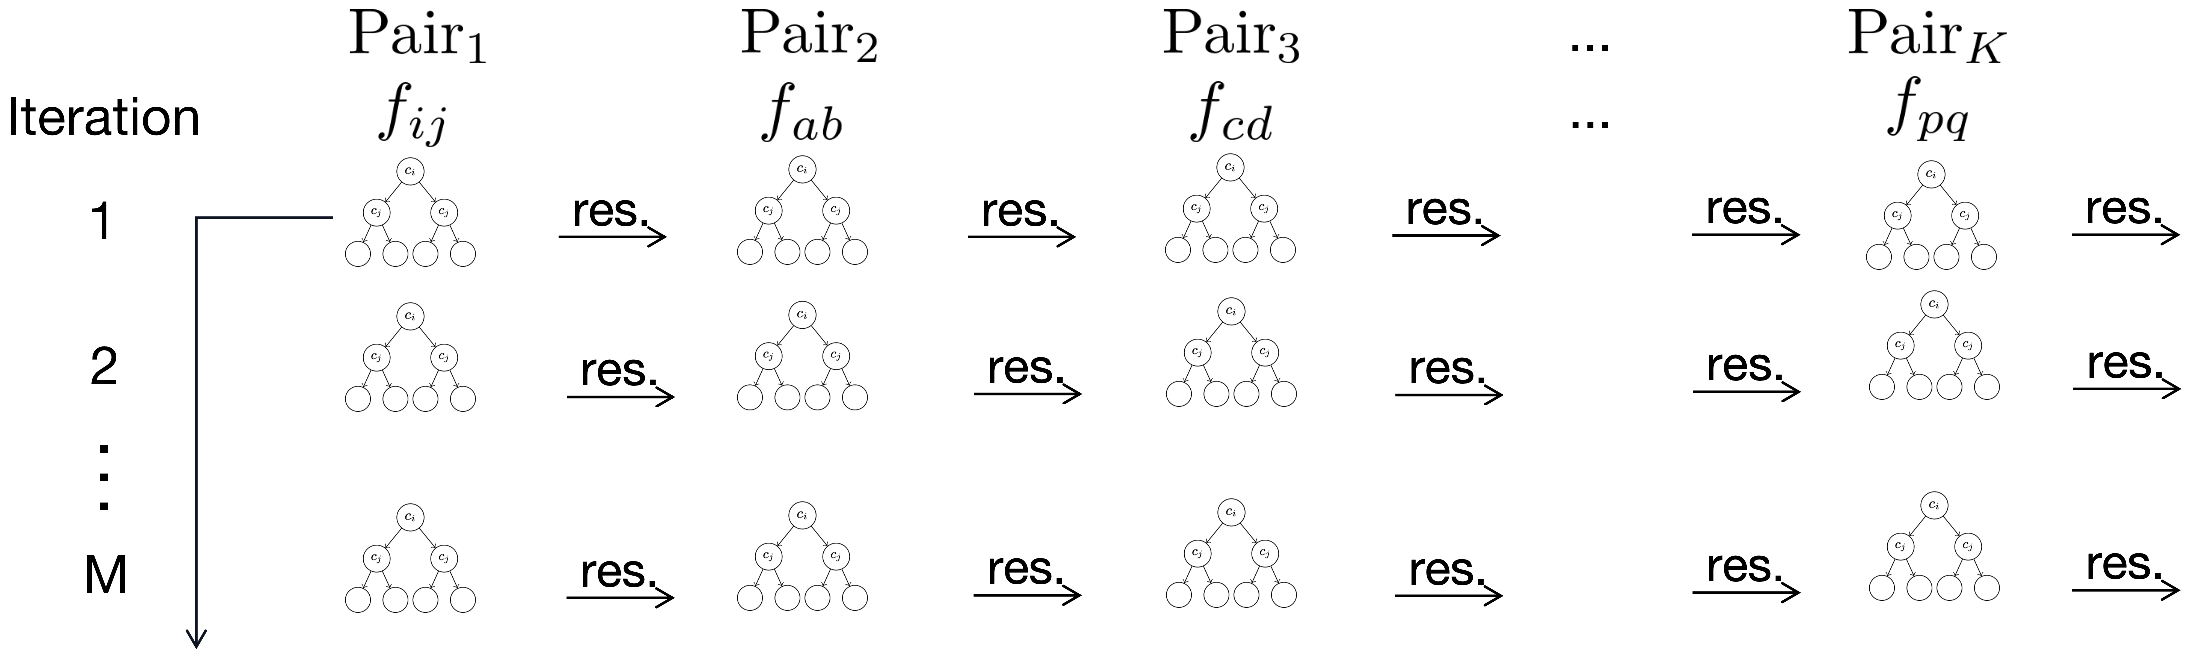
\includegraphics[width=1\linewidth]{figure/GA2M_Step1.png}
\end{frame}



\begin{frame}{Univariate EBM - Initialization}

%\textbf{Initialization:}
\begin{itemize}
    \item Set all shape functions to zero:
    $$
    f_j^{[0]}(x_j) = 0 \quad \text{for all } j = 1, \dots, p
    $$
    \item Compute initial model prediction:
    $$
    \hat{y}^{[0]} = \sum_{j=1}^p f_j^{[0]}(x_j) = 0
    $$
    \item Compute initial pseudo-residuals (e.g., for squared loss):
    $$
    \tilde{r}^{[0]} = -\frac{\partial L}{\partial \hat{y}} = y - \hat{y}^{[0]} = y
    $$
\end{itemize}

\end{frame}

\begin{frame}{Univariate EBM - First Feature Update}
\begin{figure}
    \centering
    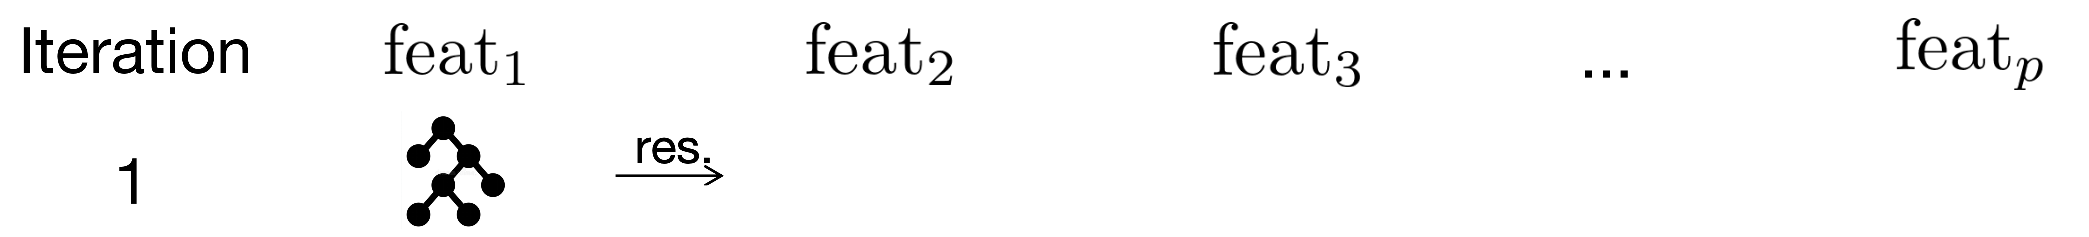
\includegraphics[width=\linewidth]{figure/EBM_Step1.png}
\end{figure}
\begin{itemize}
    \item Fit shallow bagged tree $T_1^{[1]}$ (2-4 leaves) to training data $\left\{\left(x_1, \tilde{r}^{[0]}\right)^{(i)}\right\}_{i=1}^n$\\
    $\leadsto$ Use only feature $x_1$ as input and $\tilde{r}^{[0]}$ as target
    \item Update first shape function with learning rate $\eta$:
    $$
    f_1^{[1]}(x_1) = f_1^{[0]}(x_1) + \eta \cdot T_1^{[1]}(x_1)
    $$
    \item Update prediction:
    $$
    \hat{y}^{[1]} = \sum_{j=1}^p f_j^{[1]}(x_j)
    $$
    \item Recompute pseudo-residuals:
    $$
    \tilde{r}^{[1]} =  -\frac{\partial L}{\partial \hat{y}} = y - \hat{y}^{[1]}
    $$
\end{itemize}

\end{frame}


\begin{frame}{Univariate EBM - Cycle Through Features}
\begin{figure}
    \centering
    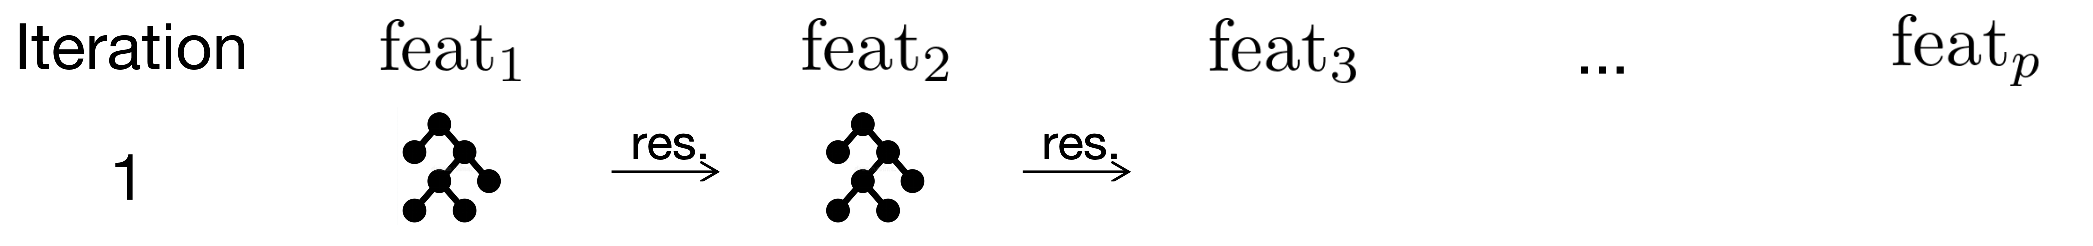
\includegraphics[width=\linewidth]{figure/EBM_Step2.png}
\end{figure}
\begin{itemize}
    \item 1st boosting iteration: \\
    Cycle through each feature $j = 2,\dots,p$:
    \begin{itemize}
        \item Fit shallow bagged tree $T_j^{[1]}$ using feature $x_j$ and previous residual $\tilde{r}^{[j-1]}$ %to $(x_j, \tilde{r}^{[j-1]})$
        \item Update $f_j$: $f_j^{[1]}(x_j) = f_j^{[0]}(x_j) + \eta \cdot T_j^{[1]}(x_j)$
        \item Recompute $\hat{y}$ and residuals: $\tilde{r}^{[j]} = y - \hat{y}^{[j]}$
    \end{itemize}
    \item After one full pass over features, we complete one boosting iteration
\end{itemize}
\end{frame}

\begin{frame}{Univariate EBM - Iterate Boosting Process}
\begin{figure}
    \centering
    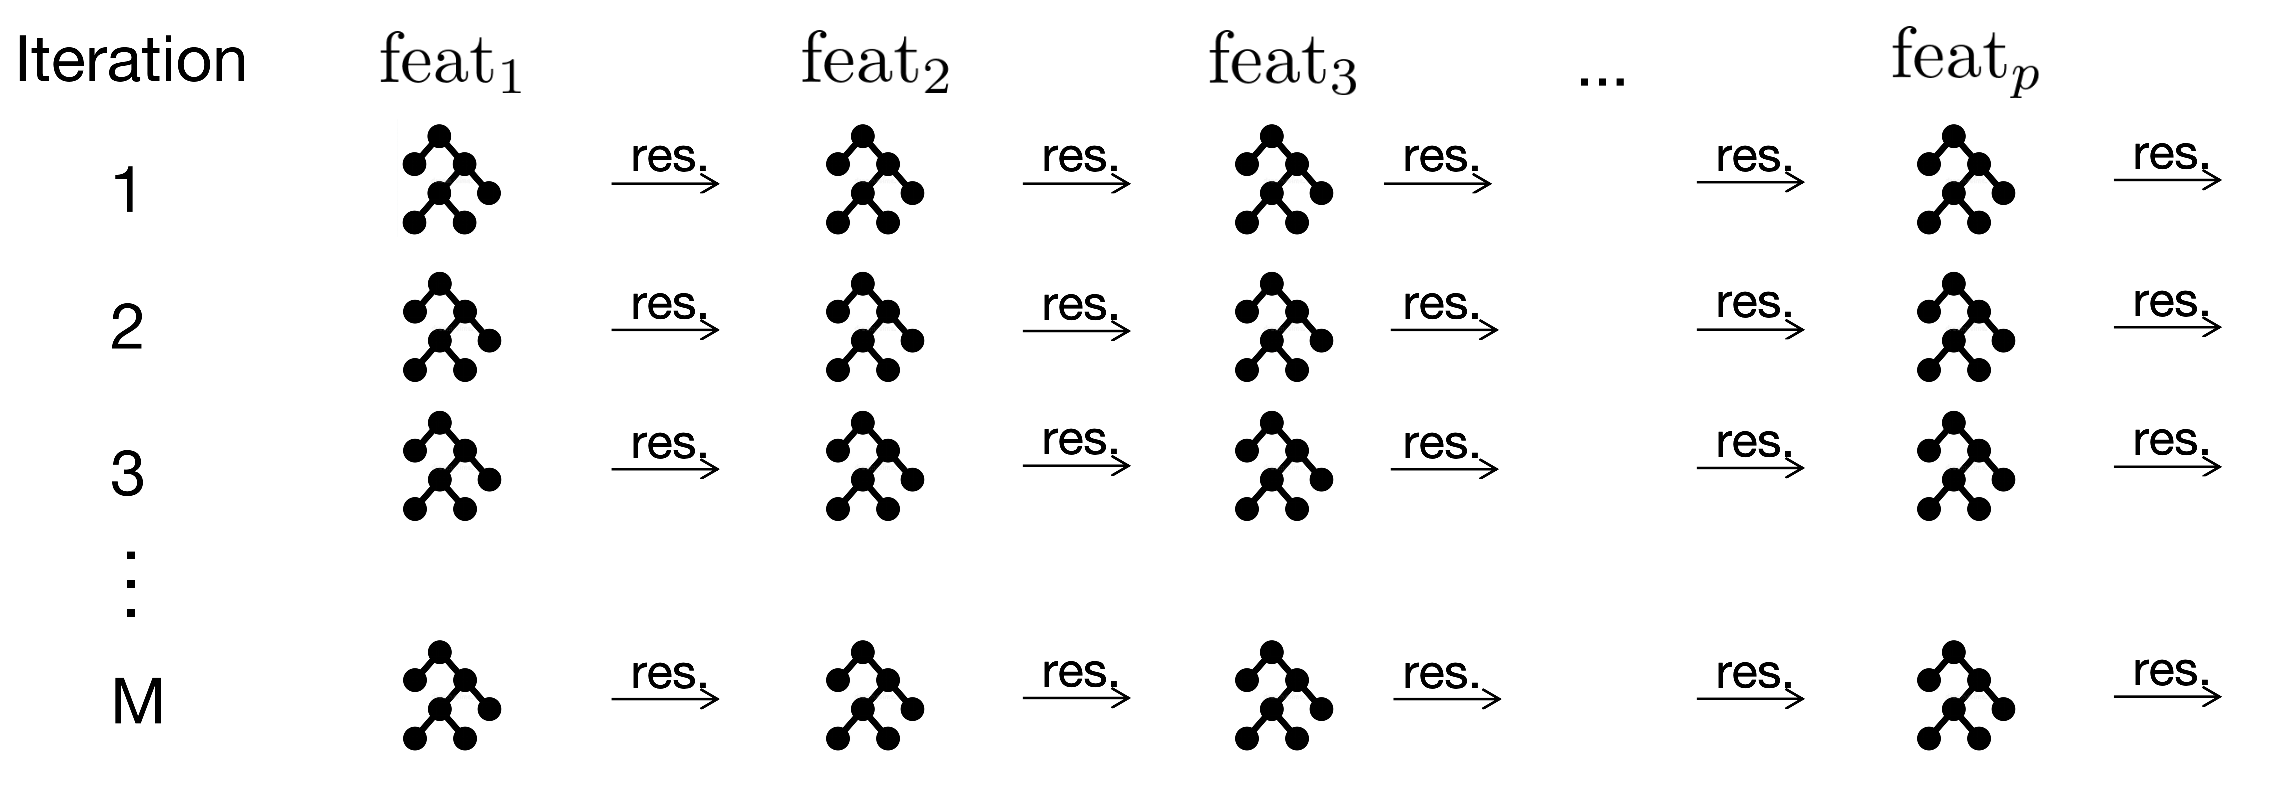
\includegraphics[width=\linewidth]{figure/EBM_Step3.png}
\end{figure}
\begin{itemize}
    \item Repeat feature-wise updates for $M$ boosting iterations (e.g., $M=10000$)
    \item In each boosting iteration:
    \begin{itemize}
        \item Cycle over all features $j=1,\dots,p$ individually %just one feature at a time 
        \item Update only one $f_j$ at a time using residuals from previous state
    \end{itemize}
    \item Use small learning rate $\eta$ to ensure smooth updates and order-invariance
\end{itemize}
\end{frame}














% \begin{frame}{Intelligible GAM - Algorithm Sketch - Part I}

% \begin{figure}
%     \centering
%     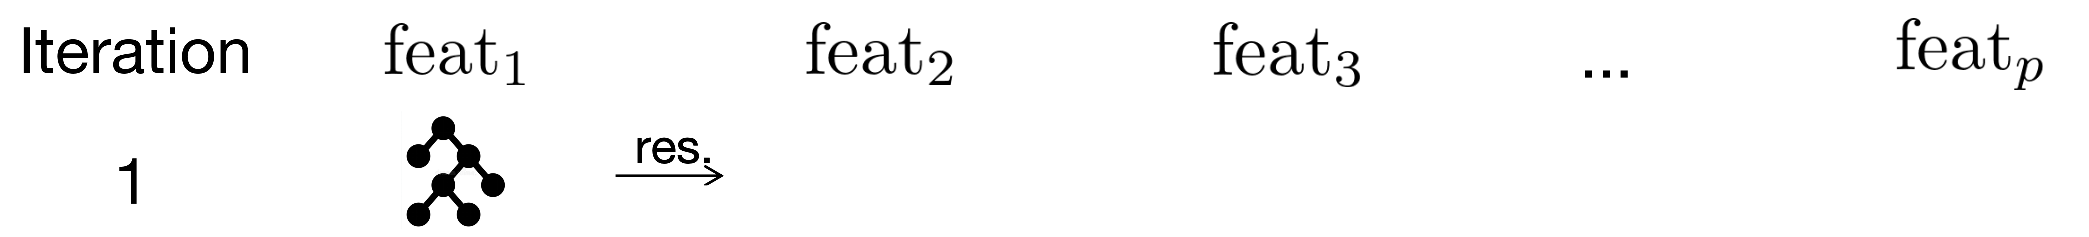
\includegraphics[width=1\linewidth]{figure/EBM_Step1.png}
%     \label{fig:Intelligible EBM_Step1}
% \end{figure}
% \begin{itemize}
%     \item Set all shape functions $f_j^{[0]}$ to zero, $j=1,\cdots,p$
%     \item Calculate the initial pseudo-residual (i.e. the negative gradient of the loss function w.r.t. the current model prediction), e.g.\\
%     1. for squared error loss: $\tilde{r}^{[0]}=-\frac{\partial L}{\partial \hat{y}}=y-\hat{y}^{[0]}=y-\sum_jf_j^{(0)}(x_{ij})$\\
%     2. for log loss: $\tilde{r}^{[0]}=-\frac{\partial L}{\partial \hat{y}}=y-\sigma(\hat{y}^{[0]})$ with $\sigma(\cdot)$ being the sigmoid function
%     \item Fit a shallow bagging tree with 2-4 leaves $T_1^{[1]}: x_{i1}\to \tilde{r}$ \textbf{only using the first feature} to predict the pseudo-residuals, with $\{x_{i1},\tilde{r}\}_1^n$ as training dataset
%     \item Update $f_1$: $f_1^{[1]}(x_{i1})=f_1^{[0]}+\eta\cdot T_1^{[1]}(x_{i1})$
%     \item Update $\hat{y}$: $\hat{y}^{[1]}=\sum_jf_j^{[1]}(x_{ij})$
%     \item Update the residual w.r.t. the original target, e.g. $\tilde{r}^{[1]}=y-\hat{y}^{[1]}$
%     \item Go to the second feature
% \end{itemize}
% \end{frame}

% \begin{frame}{Intelligible GAM - Algorithm Sketch - Part II}
% \begin{figure}
%     \centering
%     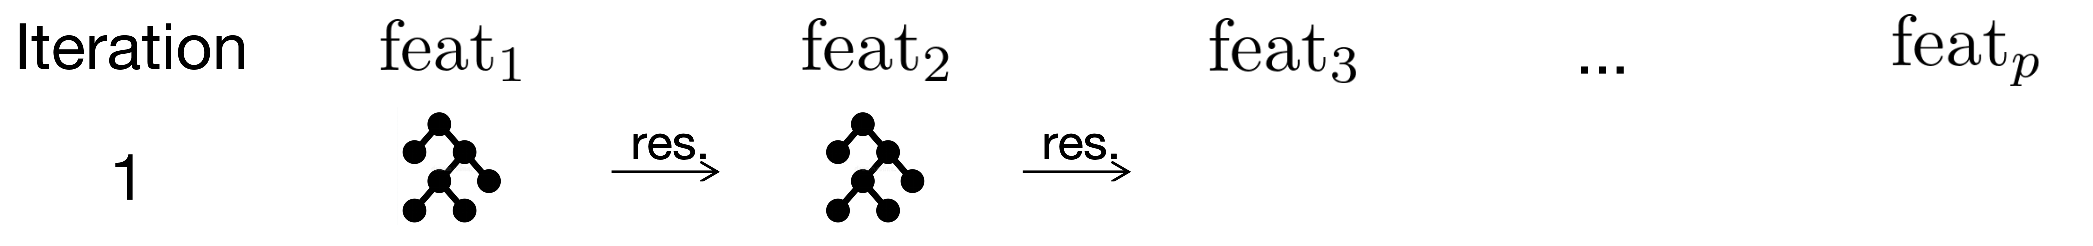
\includegraphics[width=1\linewidth]{figure/EBM_Step2.png}
%     \label{fig:Intelligible EBM_Step2}
% \end{figure}
% \begin{itemize}
%     \item Fit a shallow bagging tree $T_2^{[1]}$ \textbf{only using the second feature} to predict the updated residuals
%     \item Update $f_2$ with $f_2^{[1]}(x_{i2})=f_2^{(0)}+\eta\cdot T_2^{[1]}(x_{i2})$ and then update $\hat{y}^{[1]}$
%     \item Update the residual: this residual takes into account both what was learned on the first tree and second tree for the first two features
%     \item Go to $\text{feat}_3$
% \end{itemize}

% \end{frame}

% \begin{frame}{Intelligible GAM - Algorithm Sketch - Part III}
% \begin{figure}
%     \centering
%     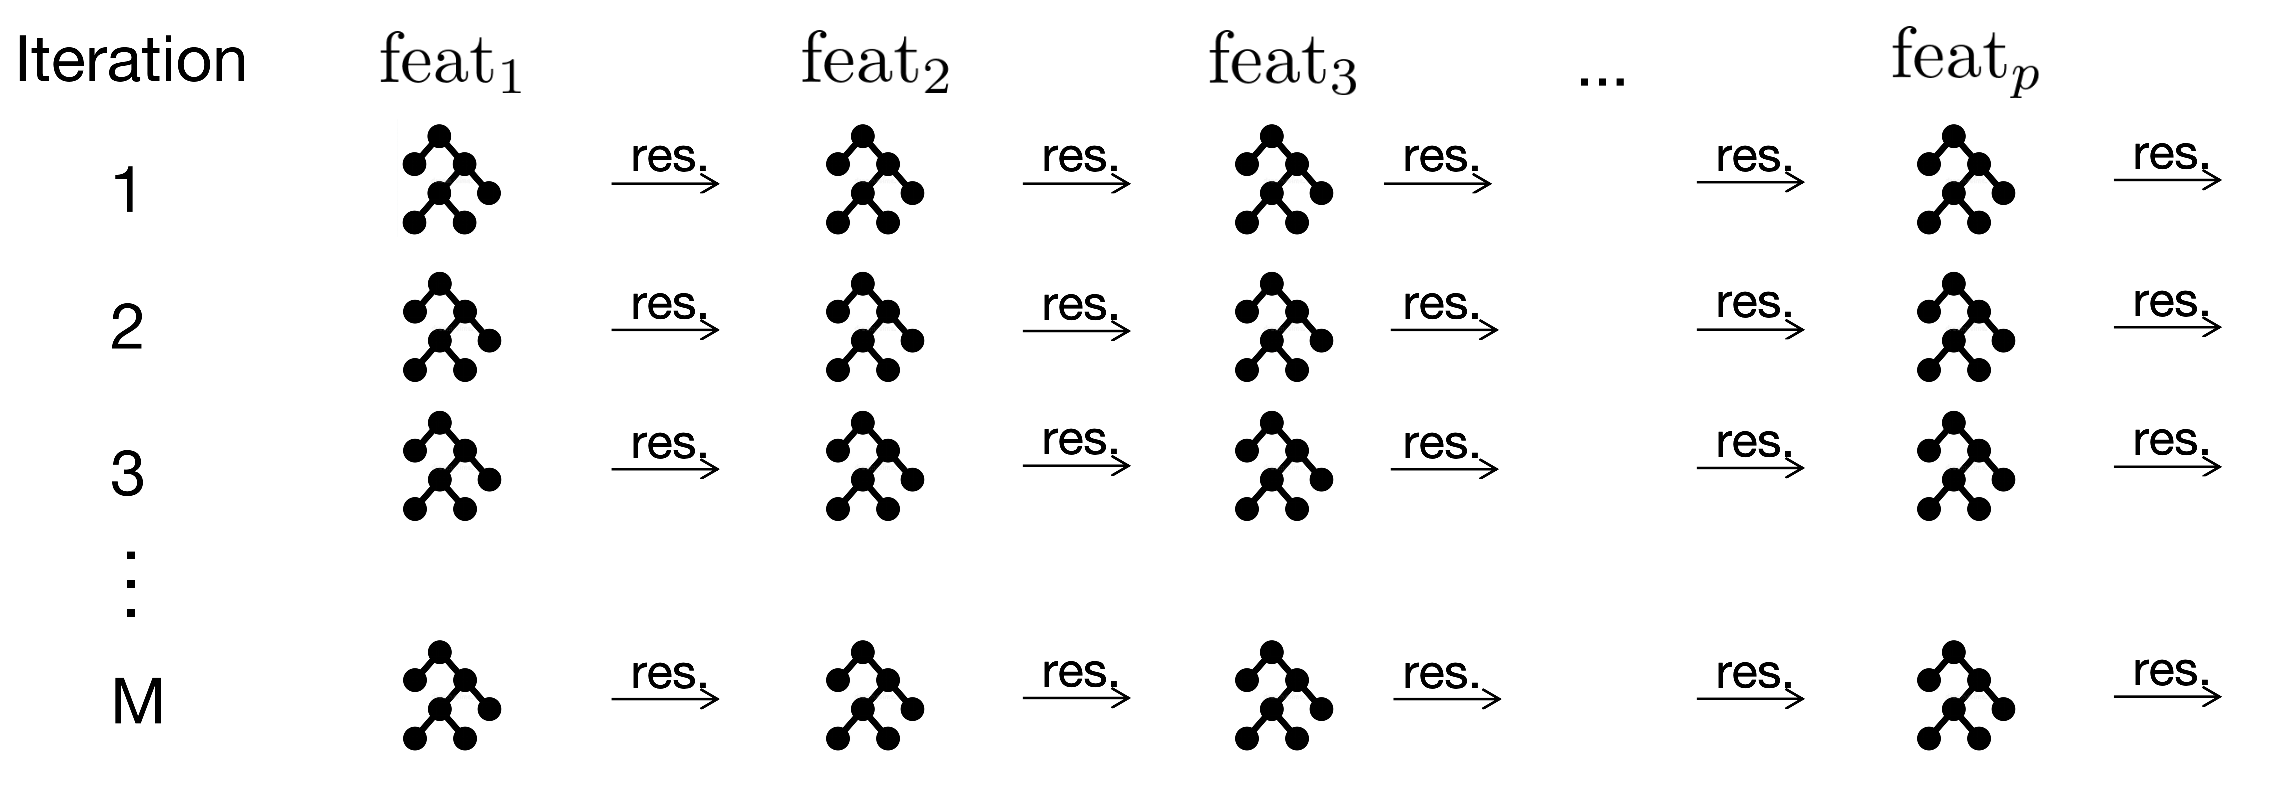
\includegraphics[width=1\linewidth]{figure/EBM_Step3.png}
%     \label{fig:Intelligible EBM_Step3}
% \end{figure}
% \begin{itemize}
%     \item Go through every feature and keep updating the residual
%     \item Grow a small tree on each feature but just one at a time in each iteration
%     \item Do $M$ iterations through these features until convergence (e.g. $M=10000$) \\
%     $\leadsto$ keep the learning rate $\eta$ so small that feature ordering does not matter
% \end{itemize}

% \end{frame}


\begin{frame}{Univariate EBM - Prediction \& Interpretability}
\begin{itemize}
    \item Final model consists of $M$ shallow trees per feature:
    $$
    \text{EBM Model} = \sum_{j=1}^p \sum_{m=1}^M \eta \cdot T_j^{[m]}(x_j)
    $$
    \item For each feature $x_j$, combine its $M$ trees into a shape function:
    $$
    \hat{f}_j(x_j) = \sum_{m=1}^M \eta \cdot T_j^{[m]}(x_j)
    $$
    \item Plot $\hat{f}_j(x_j)$ vs. $x_j$ $\leadsto$ Shows univariate marginal effect of feature $j$
    \item One plot per feature $\leadsto$ Model is fully explainable via $p$ additive plots
\end{itemize}

\medskip

\begin{figure}
    \centering
    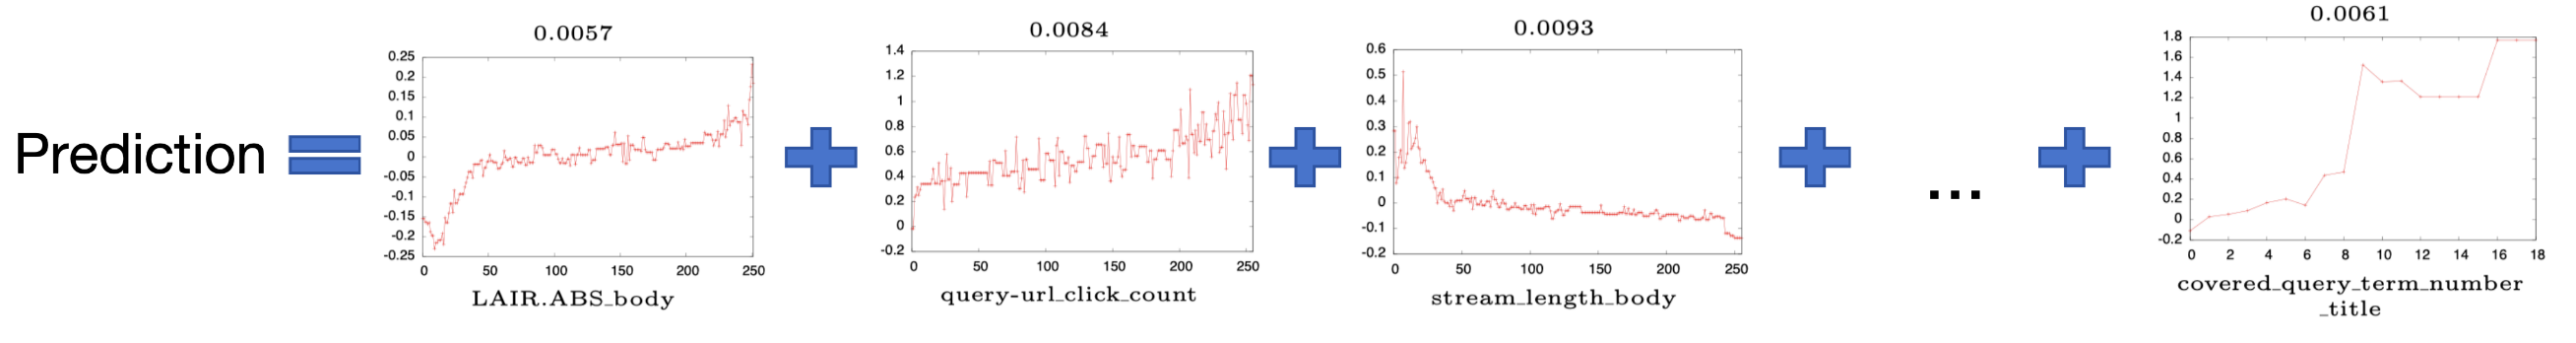
\includegraphics[width=\textwidth]{figure/ebm_prediction.png}
\end{figure}
\end{frame}


% \begin{frame}{Intelligible GAM - Prediction}
% \begin{itemize}
%     \item Output: $M$ trees which were only trained on $\text{feat}_1$ \\
%     \qquad\;\; + $M$ trees which were only trained on $\text{feat}_2$ \\
%     \qquad\;\; $\cdots$ \\
%     \qquad\;\; + $M$ trees which were only trained on $\text{feat}_p$
%     \item Summarize the weighted predictions of $M$ trees for each unique value of $\text{feat}_1$ $\hat{f}_1(x_1)=\sum_{m=1}^{M}\eta\cdot T_1^{[m]}(x_1)$, and plot $\hat{f}_1(x_1)$ vs. $x_1$ as a 2D graph
%     \item Generate a 2D graph for every feature in the same way
% \end{itemize}
% \quad $\leadsto$ Intelligible GAM: A series of 2D graphs as a perfect summary of predictions
% \begin{figure}
%     \centering
%     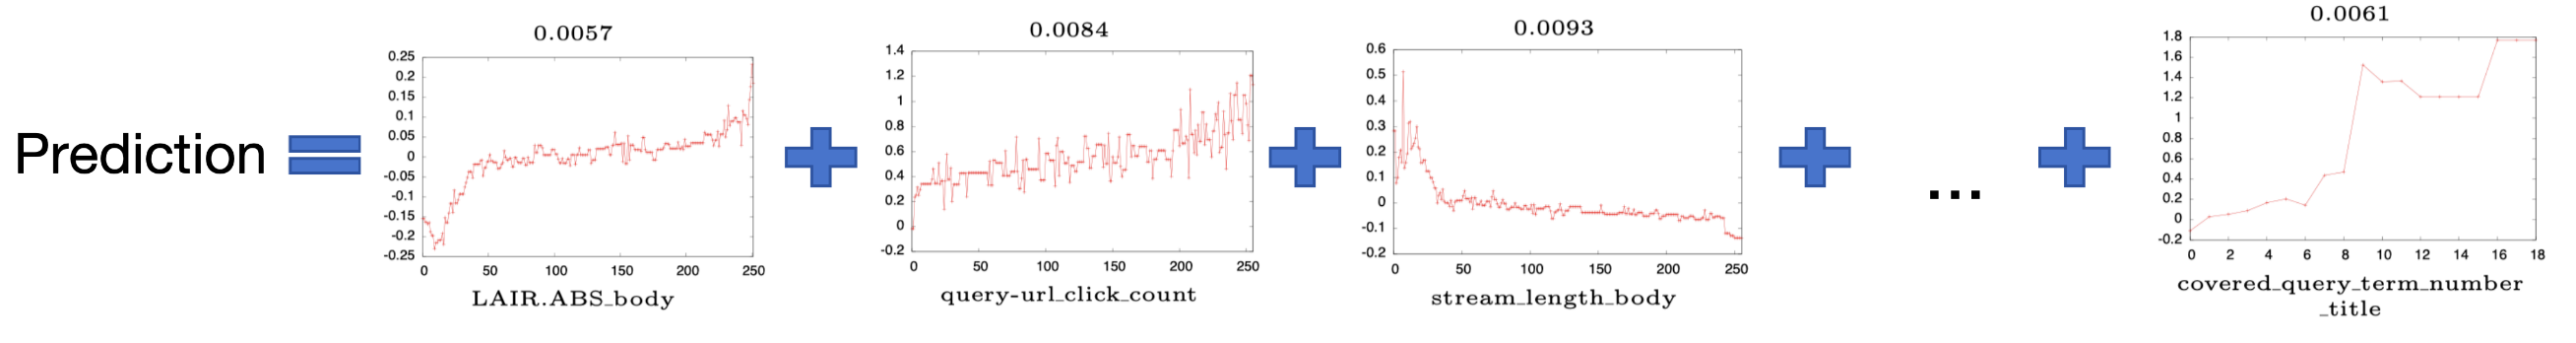
\includegraphics[width=\textwidth]{figure/ebm_prediction.png}
%     \label{fig:Intelligible ebm_prediction}
% \end{figure}
% \end{frame}

% \begin{frame}{Intelligible GAM - Novelty and Extension}
% \begin{itemize}
%     \item In each boosting step, use a bagging tree limited in size (2-4 leaves) \begin{itemize}
%         \item High accuracy, low variance, prevent overfitting
%         \item Provides discrete shape functions
%         \item Captures missing information in spline plots
%         \item High intelligibility
%     \end{itemize}
%     \item Not as accurate as unrestricted full complexity model
%     \item In the next step: % OLD
%\citebutton{Lou et al. 2013}{https://www.cs.cornell.edu/~yinlou/papers/lou-kdd13.pdf}
% new
% \furtherreading{LOU2013}
%     \begin{itemize}
%         \item Add pairwise feature interaction terms to the model
%         \item Replace the 2-4 regions of small tree
%         \item By a dynamic programming algorithm called FAST
%     \end{itemize}
% \end{itemize}
% \end{frame}

% \begin{frame}{Accurate GAM plus Pairwise Interactions}
% \textbf{Generalized Additive Models plus Interactions}: $$g(\E (y \mid \xv)) = \theta_0 + \sum f(x) + \sum f_{ij}(x,x_j)\quad for\quad i,j=1,\cdots,p,\quad i\neq j$$
% \begin{itemize}
%     \item $O(p^2)$: a large number of pairwise interactions if $p$ is big\\
%     $\leadsto$ Select only a small number of the most important interactions
%     \item Intuitively, significant reduction in RSS $\to$ Strong pair interaction
%     \item \textbf{FAST} algorithm does quick ranking without fully building every interaction function
% \end{itemize}
% \end{frame}


% \begin{frame}{GA2M - EBM \& Pairwise Interactions}
% \textbf{Generalized Additive Models plus Interactions (GA2M):}
% $$
% g\big(\mathbb{E}[y \mid \xv]\big) = \theta_0 + \sum_{j=1}^p f_j(x_j) + \sum_{i<j} f_{ij}(x_i, x_j)
% $$

% \begin{itemize}
%     \item \textbf{Extends EBM}: Adds selected bivariate functions $f_{ij}(x_i, x_j)$ to improve accuracy
%     \item \textbf{Interpretability preserved}: Each $f_{ij}$ is visualized as a 2D heatmap
%     \item Naively $O(p^2)$ possible pairs $\leadsto$ select only most relevant interactions
%     \item \textbf{FAST algorithm}: Ranks all feature pairs without exhaustively fitting them\\
%     $\leadsto$ Measures on how much a pair reduces residual sum of squares (RSS)
%     \item Top-ranked interactions added via a second-stage boosting step
% \end{itemize}
% \end{frame}

\begin{frame}{EBM with Pairwise Interactions}
\textbf{Generalized Additive Models plus Interactions (GA2M):}
$$
g\big(\mathbb{E}[y \mid \xv]\big) = \theta_0 + \sum_{j=1}^p f_j(x_j) + \sum_{i<j} f_{ij}(x_i, x_j)
$$

\begin{itemize}
    \item \textbf{Motivation}: Univariate EBM does not model interactions
    \item \textbf{Challenge}: $O(p^2)$ potential pairwise interactions
    $\leadsto$ often infeasible %to include all pairs directly
    \item \textbf{Solution - FAST algorithm} % OLD
%\citebutton{Lou et al. 2013}{https://www.cs.cornell.edu/~yinlou/papers/lou-kdd13.pdf}
% new
\furtherreading{LOU2013}:
    \begin{itemize}
        \item Efficiently estimates importance of all feature pairs
        \item Ranks pairs by reduction in residual sum of squares (RSS)
        \item Avoids fitting EBM with each pairwise interaction
    \end{itemize}
    \item \textbf{Result}: \\Add only top-ranked interactions $f_{ij}$ via asecond-stage boosting step\\
    $\leadsto$ Performed after the univariate EBM has been trained
    \item \textbf{Interpretability preserved}: Each $f_{ij}(x_i, x_j)$ visualized as a 2D heatmap
\end{itemize}
\end{frame}


% \begin{frame}{FAST Algorithm for Interaction Detection}
% \begin{columns}[c, totalwidth=\textwidth]
% \begin{column}{0.4\textwidth}
% % \begin{figure}
% %     \centering
% %     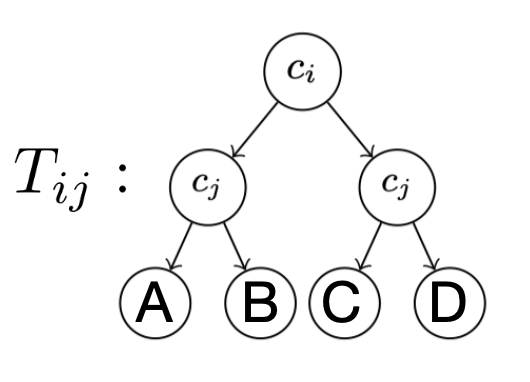
\includegraphics[width=0.8\linewidth]{figure/Tij.png}
% % \end{figure}

% \begin{figure}
% \scalebox{0.85}{
% \begin{tikzpicture}[
%   level 1/.style={sibling distance=28mm},
%   level 2/.style={sibling distance=15mm},
%   level distance=10mm,
%   every node/.style = {circle, draw, minimum size=7mm},
%   edge from parent/.style={draw,-latex}
% ]

% \node (root) {$c_i$}
%   child { node {$c_j$}
%     child { node {A} }
%     child { node {B} }
%   }
%   child { node {$c_j$}
%     child { node {C} }
%     child { node {D} }
%   };

% %\node[draw=none] at (-2.8,0.8) {$T_{ij}:$};

% \end{tikzpicture}
% }
% \end{figure}

% \end{column}
% \hfill
% \begin{column}{0.6\textwidth}
% \begin{itemize}
%     \item $T_{ij}$: Tree-like predictor with 4 leaf regions for a feature pair $(x_i, x_j)$
%     \item Define axis-aligned cut points $(c_i, c_j)$ on the sorted values of $x_i$ and $x_j$
%     \item Each split induces 4 regions: $A$, $B$, $C$, $D$
% \end{itemize}
% \end{column}
% \end{columns}

% \pause

% \begin{columns}[c, totalwidth=\textwidth]
% \begin{column}{0.4\textwidth}
% \begin{figure}
% \scalebox{0.9}{
% \begin{tikzpicture}[scale=1]

% % Rectangle dimensions
% \def\W{2.8}  % total width
% \def\H{2.8}  % total height
% \def\cx{0.9} % vertical cut
% \def\cy{1.7} % horizontal cut

% % Draw outer box and cuts
% \draw[thick] (0,0) rectangle (\W,\H);
% \draw[thick] (\cx,0) -- (\cx,\H);
% \draw[thick] (0,\cy) -- (\W,\cy);

% % Fill region a
% \fill[red!70] (0,\cy) rectangle (\cx,\H);

% % Region labels
% \node at (0.45,2.25) {$\hat{y}_A$};
% \node at (1.85,2.25) {$\hat{y}_B$};
% \node at (0.45,0.85) {$\hat{y}_C$};
% \node at (1.85,0.85) {$\hat{y}_D$};

% % Axes
% % x_j axis
% \draw[->] (0,-0.5) -- (\W+0.5,-0.5);
% \node at (0,-0.8) {small};
% \node at (\W,-0.8) {big};
% \node at (\W/2,-1.2) {$x_j$};

% % x_i axis
% \draw[->] (-0.5,0) -- (-0.5,\H+0.5);
% \node[rotate=90] at (-0.8,0) {small};
% \node[rotate=90] at (-0.8,\H) {big};
% \node[rotate=90] at (-1.2,\H/2) {$x_i$};

% % Cut point labels
% \node at (\cx,-0.3) {$c_j$};
% \node at (-0.3,\cy) {$c_i$};

% \end{tikzpicture}
% }
% \end{figure}
% \end{column}
% \hfill
% \begin{column}{0.6\textwidth}
% \begin{itemize}
%     \item Compute mean target in each region:
%     $$
%     \hat{y}_r = \frac{1}{|r|} \sum_{(\mathbf{x}, y) \in r} y, \quad r \in \{A, B, C, D\}
%     $$
%     \item Evaluate split quality via RSS:
%     %$$\text{RSS}(c_i, c_j) = \sum_{i=1}^n (y^{(i)} - \hat{y}_r^{(i)})^2$$
% $$\text{RSS}(c_i, c_j) = \sum_r \sum_{(\mathbf{x}, y) \in r} (y - \hat{y}_r)^2$$
    
%     \item Goal: find cut $(c_i, c_j)$ minimizing RSS
% \end{itemize}
% \end{column}
% \end{columns}
% \end{frame}




% \begin{frame}{FAST Algorithm for Interaction Detection}
% % For each pair of $(x_i,x_j)$ with $d_i$ and $d_j$ distinct values, calculate RSS for each possible $(c_i, c_j)$ and pick the best $T_{ij}$ with the lowest RSS ($\leadsto$ $n = d_i \cdot d_j$ different RSS values)

% For every feature pair $(x_i,x_j)$:
%       \begin{itemize}
%           \item Discretise each axis into $b\le 256$ ordered bins (uniform-width or quantile).
%           \item Evaluate all $b^{2}$ axis-aligned splits $(c_i,c_j)$ at the bin boundaries.
%       \end{itemize}


% \begin{columns}[c, totalwidth=\textwidth]
%     \begin{column}{0.45\textwidth}
% \[
%         \begin{array}{@{}l@{\quad}l@{\quad}l@{\quad}l@{\quad}l}
%     \begin{tikzpicture}[baseline=(current bounding box.center)]
%         \draw (0,0) rectangle (1.2,1.2);
%         \draw (0.4,0) -- (0.4,1.2); 
%         \draw (0,0.8) -- (1.2,0.8); 
%         \node at (0.2,0.4) {C};
%         \node at (0.8,0.4) {D};
%         \node at (0.2,1) {A};
%         \node at (0.8,1) {B};
%     \end{tikzpicture} & \text{$\Rightarrow$} & \begin{tikzpicture}[baseline=(current bounding box.center)]
%         \draw (0,0) rectangle (1.2,1.2);
%         \draw (0.4,0) -- (0.4,1.2); 
%         \draw (0,0.8) -- (1.2,0.8); 
%         \node at (0.2,0.4) {$\hat{y}_C$};
%         \node at (0.8,0.4) {$\hat{y}_D$};
%         \node at (0.2,1) {$\hat{y}_A$};
%         \node at (0.8,1) {$\hat{y}_B$};
%     \end{tikzpicture} & \text{$\Rightarrow$} & \text{$RSS_1$}\\[0.7cm] 
%     \begin{tikzpicture}[baseline=(current bounding box.center)]
%         \draw (0,0) rectangle (1.2,1.2);
%         \draw (0.6,0) -- (0.6,1.2); 
%         \draw (0,0.6) -- (1.2,0.6); 
%         \node at (0.3,0.3) {C};
%         \node at (0.9,0.3) {D};
%         \node at (0.3,0.9) {A};
%         \node at (0.9,0.9) {B};
%     \end{tikzpicture} & \text{$\Rightarrow$} & \begin{tikzpicture}[baseline=(current bounding box.center)]
%         \draw (0,0) rectangle (1.2,1.2);
%         \draw (0.6,0) -- (0.6,1.2); 
%         \draw (0,0.6) -- (1.2,0.6); 
%         \node at (0.3,0.3) {$\hat{y}_C$};
%         \node at (0.9,0.3) {$\hat{y}_D$};
%         \node at (0.3,0.9) {$\hat{y}_A$};
%         \node at (0.9,0.9) {$\hat{y}_B$};
%     \end{tikzpicture} & \text{$\Rightarrow$} & \text{$RSS_2$}\\[0.7cm] 
%     \makebox[1cm][c]{\vdots} & & \makebox[1cm][c]{\vdots} & & \makebox[1cm][c]{\vdots}\\[0.3cm]
%     \begin{tikzpicture}[baseline=(current bounding box.center)]
%         \draw (0,0) rectangle (1.2,1.2);
%         \draw (0.8,0) -- (0.8,1.2); 
%         \draw (0,0.4) -- (1.2,0.4); 
%         \node at (0.4,0.2) {C};
%         \node at (1,0.2) {D};
%         \node at (0.4,0.8) {A};
%         \node at (1,0.8) {B};
%     \end{tikzpicture} & \text{$\Rightarrow$} & \begin{tikzpicture}[baseline=(current bounding box.center)]
%         \draw (0,0) rectangle (1.2,1.2);
%         \draw (0.8,0) -- (0.8,1.2); 
%         \draw (0,0.4) -- (1.2,0.4); 
%         \node at (0.4,0.2) {$\hat{y}_C$};
%         \node at (1,0.2) {$\hat{y}_D$};
%         \node at (0.4,0.8) {$\hat{y}_A$};
%         \node at (1,0.8) {$\hat{y}_B$};
%     \end{tikzpicture} & \text{$\Rightarrow$} & \text{$RSS_{b^2}$}\\ 
% \end{array}
% \]
%     \end{column}
%         \begin{column}{0.53\textwidth}
%         For each candidate cut $(c_i, c_j)$:
%   \begin{itemize}
%     \item Divide 2D input space into 4 quadrants: A, B, C, D
%     \item Compute average target $\hat{y}_r$ in each region $r \in \{A, B, C, D\}$
%     \item Predict using a constant in each region
%     \item Compute total RSS of this piecewise predictor
%   \end{itemize}
% Select the cut with minimal RSS - its value quantifies the interaction strength of $(x_i, x_j)$

%     \end{column}
% \end{columns}
% % \medskip
% % \textbf{Why is this fast?}\\
% % Precompute cumulative sums (targets and counts) over sorted features\\
% % $\leadsto$ Fast lookup of region totals for any cut $(c_i, c_j)$ without scanning data


% %\text{\parbox[t]{6cm}{Select the lowest RSS and measure interaction strength of $(x_i, x_j)$ via risk reduction}}
% \end{frame}



% \begin{frame}{RSS in FAST: Region-Based Derivation}

% \textbf{Goal:} Efficiently compute RSS over $r \in \{A, B, C, D\}$ defined by cuts $(c_i, c_j)$

% \textbf{Step 1: Expand squared residuals}
% \[
% \text{RSS}(c_i, c_j) = \sum_{r} \sum_{(x, y) \in r} (y - \hat{y}_r)^2
% = \sum_{r} \left( \sum y^2 - 2 \hat{y}_r \sum y + \hat{y}_r^2 \cdot n_r \right)
% \]

% \textbf{Step 2: Define region-wise statistics}
% \[
% \mu_r = \frac{S_r}{n_r}, \quad
% S_r = \sum_{(x, y) \in r} y, \quad
% Q_r = \sum_{(x, y) \in r} y^2, \quad
% n_r = |r|
% \]

% \textbf{Step 3: Substitute and simplify}
% \[
% \text{RSS}(c_i, c_j) = \sum_r \left( Q_r - \frac{S_r^2}{n_r} \right)
% \]

% \textbf{Why is this fast?}
% \begin{itemize}
%     \item Precompute cumulative sums of $y$, $y^2$, and counts
%     \item Allows fast lookup of $S_r$, $Q_r$, and $n_r$ for any rectangle defined by $(c_i, c_j)$
% \end{itemize}


% \end{frame}






\begin{frame}{FAST: Pair-wise Interaction Strength}

We evaluate a 4-leaf, axis-aligned tree $T_{ij}$ over the 2D feature projection $(x_i, x_j)$.

\begin{columns}[T,totalwidth=\textwidth]
% ----- left: predictor diagram ---------------------------------
\begin{column}{0.4\textwidth}\centering
\only<1>{

\begin{figure}
\scalebox{0.85}{
\begin{tikzpicture}[
  level 1/.style={sibling distance=28mm},
  level 2/.style={sibling distance=15mm},
  level distance=10mm,
  every node/.style = {circle, draw, minimum size=7mm},
  edge from parent/.style={draw,-latex}
]

\node (root) {$c_i$}
  child { node {$c_j$}
    child { node {A} }
    child { node {B} }
  }
  child { node {$c_j$}
    child { node {C} }
    child { node {D} }
  };

%\node[draw=none] at (-2.8,0.8) {$T_{ij}:$};

\end{tikzpicture}
}
\end{figure}

\begin{tikzpicture}[scale=0.9,baseline=(current bounding box.center)]
% outer box
\draw[thick] (0,0) rectangle (3,3);
% axis-aligned cuts
\def\xc{1.2}\def\yc{1.9}
\draw[thick] (\xc,0)--(\xc,3);
\draw[thick] (0,\yc)--(3,\yc);
% region labels
\node at (0.6,2.5) {$A$};
\node at (2.1,2.5) {$B$};
\node at (0.6,0.9) {$C$};
\node at (2.1,0.9) {$D$};
% axis labels
\node[below] at (1.5,-0.4) {$x_j$};
\node[rotate=90] at (-0.6,1.5) {$x_i$};
% cut labels
\node[below] at (\xc,0) {$c_j$};
\node[left]  at (0,\yc) {$c_i$};
\end{tikzpicture}

{\small tree $T_{ij}$ with 4 leaves}
}

\only<2>{
\[
\begin{array}{@{}l@{\hskip 0.6em}l@{\hskip 0.6em}l@{\hskip 0.6em}l@{\hskip 0.6em}l}
    \begin{tikzpicture}[baseline=(current bounding box.center)]
        \draw (0,0) rectangle (1.2,1.2);
        \draw (0.4,0) -- (0.4,1.2); 
        \draw (0,0.8) -- (1.2,0.8); 
        \node at (0.2,0.4) {C};
        \node at (0.8,0.4) {D};
        \node at (0.2,1) {A};
        \node at (0.8,1) {B};
    \end{tikzpicture} & \text{$\Rightarrow$} & \begin{tikzpicture}[baseline=(current bounding box.center)]
        \draw (0,0) rectangle (1.2,1.2);
        \draw (0.4,0) -- (0.4,1.2); 
        \draw (0,0.8) -- (1.2,0.8); 
        \node at (0.2,0.4) {$\hat{y}_C$};
        \node at (0.8,0.4) {$\hat{y}_D$};
        \node at (0.2,1) {$\hat{y}_A$};
        \node at (0.8,1) {$\hat{y}_B$};
    \end{tikzpicture} & \text{$\Rightarrow$} & \text{$RSS_1$}\\[0.7cm] 
    \begin{tikzpicture}[baseline=(current bounding box.center)]
        \draw (0,0) rectangle (1.2,1.2);
        \draw (0.6,0) -- (0.6,1.2); 
        \draw (0,0.6) -- (1.2,0.6); 
        \node at (0.3,0.3) {C};
        \node at (0.9,0.3) {D};
        \node at (0.3,0.9) {A};
        \node at (0.9,0.9) {B};
    \end{tikzpicture} & \text{$\Rightarrow$} & \begin{tikzpicture}[baseline=(current bounding box.center)]
        \draw (0,0) rectangle (1.2,1.2);
        \draw (0.6,0) -- (0.6,1.2); 
        \draw (0,0.6) -- (1.2,0.6); 
        \node at (0.3,0.3) {$\hat{y}_C$};
        \node at (0.9,0.3) {$\hat{y}_D$};
        \node at (0.3,0.9) {$\hat{y}_A$};
        \node at (0.9,0.9) {$\hat{y}_B$};
    \end{tikzpicture} & \text{$\Rightarrow$} & \text{$RSS_2$}\\[0.7cm] 
    \makebox[1cm][c]{\vdots} & & \makebox[1cm][c]{\vdots} & & \makebox[1cm][c]{\vdots}\\[0.3cm]
    \begin{tikzpicture}[baseline=(current bounding box.center)]
        \draw (0,0) rectangle (1.2,1.2);
        \draw (0.8,0) -- (0.8,1.2); 
        \draw (0,0.4) -- (1.2,0.4); 
        \node at (0.4,0.2) {C};
        \node at (1,0.2) {D};
        \node at (0.4,0.8) {A};
        \node at (1,0.8) {B};
    \end{tikzpicture} & \text{$\Rightarrow$} & \begin{tikzpicture}[baseline=(current bounding box.center)]
        \draw (0,0) rectangle (1.2,1.2);
        \draw (0.8,0) -- (0.8,1.2); 
        \draw (0,0.4) -- (1.2,0.4); 
        \node at (0.4,0.2) {$\hat{y}_C$};
        \node at (1,0.2) {$\hat{y}_D$};
        \node at (0.4,0.8) {$\hat{y}_A$};
        \node at (1,0.8) {$\hat{y}_B$};
    \end{tikzpicture} & \text{$\Rightarrow$} & \text{$RSS_{b^2}$}\\ 
\end{array}
\]
}
\end{column}
% ----- right: algorithm steps ----------------------------------
\begin{column}{0.6\textwidth}
\small
\begin{enumerate}\itemsep4pt
  \item<1-> {\bf Discretize}\,: Map each axis to \(b\!\le\!256\) ordered
        bins (quantile or equal-width).
  \item<2-> {\bf Iterate} over \(b^{2}\) candidate cuts
        \((c_i,c_j)\). %at bin boundaries.
  \item<2-> {\bf Fit}\,: For each cut, assign a constant
        \(\hat y_r\!=\!\text{mean}(y\!\in\!r)\) to
        \(r\!\in\!\{A,B,C,D\}\).
  \item<2-> {\bf Compute RSS summed over all regions}:   
  {\footnotesize
  \[
\begin{aligned}
\text{RSS}(c_i, c_j) 
&= \sum_{r} \sum_{(x,y) \in r} (y - \hat{y}_r)^2 \\
&= \sum_{r} \left( \sum_{(x,y) \in r} y^2 - \frac{1}{n_r} \left(\sum_{(x,y) \in r} y \right)^2 \right)
%\sum_{r} \left( \sum_{(x,y) \in r} y^2 - 2 \hat{y}_r \sum_{(x,y) \in r} y + \hat{y}_r^2 \cdot n_r \right)
\end{aligned}
\]
        % \(\text{RSS}(c_i,c_j)=\sum_{r}
        %  \sum_{(x,y)\in r}(y-\hat y_r)^{2}
        %  \)
         
 % \(\text{RSS}_0\;=\;\sum_{i=1}^{n}\bigl(y_k-\bar y\bigr)^2
 %              =\sum_{i}y_k^{2}-\frac{T^{2}}{n}\)
              
 % \(\Delta\text{RSS}(c_i,c_j) =\text{RSS}_0-\text{RSS}(c_i,c_j)\)
 }
  \item<2-> {\bf Select}\,: Keep the split with minimal RSS.\\
  $\leadsto$ largest RSS drop = strongest interaction. \\% of \((x_i,x_j)\) \\
  %$\leadsto$ $\mathcal{O}(n+b^{2})$ per pair.
\end{enumerate}

\end{column}
\end{columns}
\end{frame}











\begin{frame}{FAST: Use RSS Drop}
\small

To evaluate a cut pair $(c_i, c_j)$, we use precomputed per-region statistics:

\begin{itemize}
  \item For each region $r \in \{A, B, C, D\}$, compute:
    \[
    S_r = \sum_{(x,y)\in r} y,\quad
    %Q_r = \sum_{(x,y)\in r} y^2,\quad
    n_r = |\{(x,y)\in r\}|,\quad
    \hat y_r = S_r / n_r
    \]
  \item Plug into RSS summed over all regions: $$
\text{RSS}(c_i, c_j) = \sum_{r} \left( \sum_{(x,y) \in r} y^2 - \frac{1}{n_r} \left(\sum_{(x,y) \in r} y \right)^2 \right) = 
%\sum_{r}\!\left(\sum_{(x,y)\in r} y^2-\frac{S_r^{2}}{n_r}\right)
\sum_{r}\sum_{(x,y)\in r} y^2+\sum_{r}\frac{S_r^{2}}{n_r}
$$
  %\item Requires only scalar summaries $(S_r, Q_r, n_r)$
  %\item No access to individual samples needed at scoring time
  %\item Baseline (unsplit) RSS: $\text{RSS}_0 = \sum_k y_k^2 - \frac{T^2}{n}$, with $T = \sum_k y_k$ and $\bar y = T/n$
  \item 
For a candidate cut, compute \textbf{RSS drop}:
\begin{align*}
  \Delta\text{RSS}(c_i,c_j)
     &=\text{RSS}_{\text{parent}}-\text{RSS}(c_i,c_j)\\
     &=\left(\sum_{i = 1}^n \left(y^{(i)}\right)^{2} -\frac{S_n^{2}}{n}\right)
       -  \sum_{r}\sum_{(x,y)\in r} y^2+\sum_{r}\frac{S_r^{2}}{n_r}
\end{align*}
\end{itemize}


\end{frame}
% ============================================================================
\begin{frame}{FAST: Use RSS drop}

Because $\sum_{i = 1}^n \left(y^{(i)}\right) ^{2} = \sum_{r}\sum_{(x,y)\in r} y^2$, \emph{all squared target terms cancel}:
\[
  \boxed{\displaystyle
  \Delta\text{RSS}(c_i,c_j)
     =\sum_{r}\frac{S_r^{2}}{n_r}\;-
      \frac{S_n^{2}}{n}}
\]
The parent term $S_n^{2}/n$ is constant across all cuts.  Hence
\[
  \textbf{maximize }\Delta\text{RSS}(c_i,c_j)=\sum_{r}\frac{S_r^{2}}{n_r}
  \quad\Longleftrightarrow\quad
  \textbf{minimize }\text{RSS}(c_i,c_j).
\]


\textbf{Why is this efficient?}
\begin{itemize}
  \item Precompute cummulative sums of \(y\) and counts across the binned grid
  \item Enables fast lookup of region statistics \(S_r, n_r\) for any cut
  \item No additional data scan or recomputation needed across the \(b^2\) candidate cuts
  \item For the best cut: Compare and select the largest
$\Delta\text{RSS}(c_i,c_j)$.
\end{itemize}


\end{frame}

% % ============================================================================
% \begin{frame}{Step 4: FAST search in $\mathcal O(b^2)$ per pair}
% \small
% \begin{enumerate}\itemsep4pt
%   \item \textbf{Discretise}: map each feature axis to $b\,(\le256)$ bins.
%   \item \textbf{Iterate}: enumerate the $b^{2}$ cut pairs $(c_i,c_j)$.
%   \item \textbf{Lookup stats}: obtain $(S_r,n_r)$ for the four rectangles
%         in $O(1)$s.
%   \item \textbf{Score}: compute $S(c_i,c_j)=\sum_{r}S_r^{2}/n_r$.
%   \item \textbf{Select}: keep the cut with the \emph{largest} $S$ (largest
%         RSS drop).
% \end{enumerate}
% \medskip
% %Overall cost per feature pair: $\mathcal O(n+b^{2})$ preprocessing for thevcumulative tables, then $\mathcal O(b^{2})$ scoring.
% \end{frame}















% \begin{frame}{FAST: constant-region RSS in closed form}

% \small
% \textbf{Pre-compute for every rectangle}  
% \(r\in\{A,B,C,D\}\):
% \[
% S_r=\!\!\sum_{(x,y)\in r}\!y, \qquad 
% Q_r=\!\!\sum_{(x,y)\in r}\!y^{2}, \qquad 
% n_r=|r|, \qquad
% y_r=\frac{S_r}{n_r}.
% \]

% \medskip
% \textbf{RSS:}

% \[
% \text{RSS}(c_i, c_j) = \sum_{r} \sum_{(x, y) \in r} (y - \hat{y}_r)^2
% = \sum_{r} \left( \sum y^2 - 2 \hat{y}_r \sum y + \hat{y}_r^2 \cdot n_r \right)
% \]

% \medskip
% \textbf{Plug into RSS:}
% \[
% \text{RSS}(c_i,c_j)=
% \sum_{r}\!\left(
%       Q_r-\frac{S_r^{2}}{n_r}\right).
% \]

% \medskip
% \textbf{Why is this fast?}
% \begin{itemize}
%   \item Precompute cummulative sums of \(y\), \(y^2\), and counts across the binned grid
%   \item Enables fast lookup of region statistics \(S_r, Q_r, n_r\) for any cut
%   \item No additional data scan or recomputation needed across the \(b^2\) candidate cuts
% \end{itemize}

% % \vspace{1ex}
% % \hfill{\footnotesize Lou et al.\ 2013, §4.1}
% \end{frame}










% \begin{frame}{FAST feature interaction detection - PART I}

% \begin{columns}[T, totalwidth=\textwidth]
% \begin{column}{0.5\textwidth}
% \begin{figure}
%     \centering
%     \includegraphics[width=0.6\linewidth]
%     {figure/Tij.png}
%     \label{fig:tree-like predictor}
% \end{figure}
% \begin{figure}
%     \centering
%     \includegraphics[width=0.65\linewidth]
%     {figure/FAST1.png}
%     \label{fig:FAST1}
% \end{figure}
% \end{column}
% \hfill
% \centering
% \begin{column}{0.6\textwidth}
% \begin{itemize}
%     \item $T_{ij}$: A tree-like interaction predictor with 4 leaves for each pair of features
%     \item $c$, $c_j$: One cut (grid point) on the \textbf{sorted} values of feature $x$ and $x_j$, respectively
%     \item $A$, $B$, $C$, $D$: Notation for 4 leaf regions
%     \item \textbf{Idea}: Search for all possible $(c, c_j)$ and pick the best $T_{ij}$ with the lowest RSS
%     \item Prediction value on region r, $r\in\{A, B, C, D\}$:
%     $$\hat{y}_r=T_{ij}.r=\frac{1}{\vert r\vert}\sum_{(\mathbf{x},y)\in r}y=\frac{\text{Sum of targets in }r}{\text{Sum of counts in }r}$$
%     \item $\text{RSS}=\sum_{k=1}^n(y_k-T_{ij}(\mathbf{x}_k))^2$ \\
%     \qquad\;$=\sum_{k=1}^Ny_k^2-2\sum_r\left(\hat{y}_r\cdot\sum_{(\mathbf{x},y)\in r}y\right)$\\
%     \qquad\;\;\;\;$+\sum_r\hat{y}_r^2\cdot\vert r\vert$
% \end{itemize}
% \end{column}
% \end{columns}

% \end{frame}

% \begin{frame}{FAST feature interaction detection - PART II}

% \begin{columns}[T, totalwidth=\textwidth]
% \begin{column}{0.5\textwidth}
% \begin{itemize}
% \item How to quickly get sum of targets and sum of counts for all possible cuts?\\
%     $\leadsto$ Use \textbf{marginal cumulative histograms} (CH)
% \end{itemize}
% \begin{figure}
%     \centering
%     \includegraphics[width=\linewidth]
%     {figure/FAST.png}
%     \\An illustration for computing sum of targets for each quadrant
%     \label{fig:FAST2}
% \end{figure}
% \end{column}
% \hfill
% \centering
% \begin{column}{0.6\textwidth}
% \begin{itemize}
%     \item For example:\\
%     $CH_j^t(c_j)$: cumulative sum of targets for data points with $x_j\leq c_j$;\\
%     $\overline{CH_j^t }(c_j)$: cumulative sum of targets for data points with $x_j>c_j$
%     \item Create \textbf{two lookup tables} to store values for every $(c, c_j)$, :\\
%     1. Compute the cumulative sum of targets in four regions, and store the values in the \textbf{table of targets} $L^t(c,c_j)=[a,b,c,d]$\\
%     2. Compute the cumulative sum of counts in four regions, and store the values in the \textbf{table of counts} $L^w(c,c_j)=[a,b,c,d]$
%     \item Given any $(c, c_j)$, values of $(b,c,d)$ can be easily derived with known $\color{red}a$\\
%     $\leadsto$Construct lookup tables using dynamic programming
% \end{itemize}
% \end{column}
% \end{columns}

% \end{frame}

% \begin{frame}{FAST feature interaction detection - PART III}

% \begin{itemize}
%     \item For $x$ with $d$ possible values and $x_j$ with $d_j$ possible values:\\
%     $\leadsto$ compute and store $dd_j$ records of $[a,b,c,d]$ in both table of targets and table of counts
%     \item For each pair of $(x,x_j)$, calculate RSS for each possible $(c, c_j)$ and pick the best $T_{ij}$ with the lowest RSS [Note: $\hat{y}_A$ can be simply calculated as $L^t(c,c_j).a/L^w(c,c_j).a$]
% \end{itemize}
% \[
% \text{\qquad$dd_j$ possible $(c, c_j)$}
% \left\{
% \begin{array}{@{}l@{\quad}l@{\quad}l@{\quad}l@{\quad}l}
%     \begin{tikzpicture}[baseline=(current bounding box.center)]
%         \draw (0,0) rectangle (1.2,1.2);
%         \draw (0.4,0) -- (0.4,1.2); 
%         \draw (0,0.8) -- (1.2,0.8); 
%         \node at (0.2,0.4) {c};
%         \node at (0.8,0.4) {d};
%         \node at (0.2,1) {a};
%         \node at (0.8,1) {b};
%     \end{tikzpicture} & \text{$\Rightarrow$} & \begin{tikzpicture}[baseline=(current bounding box.center)]
%         \draw (0,0) rectangle (1.2,1.2);
%         \draw (0.4,0) -- (0.4,1.2); 
%         \draw (0,0.8) -- (1.2,0.8); 
%         \node at (0.2,0.4) {$\hat{y}_C$};
%         \node at (0.8,0.4) {$\hat{y}_D$};
%         \node at (0.2,1) {$\hat{y}_A$};
%         \node at (0.8,1) {$\hat{y}_B$};
%     \end{tikzpicture} & \text{$\Rightarrow$} & \text{$RSS_1$}\\[0.7cm] 
%     \begin{tikzpicture}[baseline=(current bounding box.center)]
%         \draw (0,0) rectangle (1.2,1.2);
%         \draw (0.6,0) -- (0.6,1.2); 
%         \draw (0,0.6) -- (1.2,0.6); 
%         \node at (0.3,0.3) {c};
%         \node at (0.9,0.3) {d};
%         \node at (0.3,0.9) {a};
%         \node at (0.9,0.9) {b};
%     \end{tikzpicture} & \text{$\Rightarrow$} & \begin{tikzpicture}[baseline=(current bounding box.center)]
%         \draw (0,0) rectangle (1.2,1.2);
%         \draw (0.6,0) -- (0.6,1.2); 
%         \draw (0,0.6) -- (1.2,0.6); 
%         \node at (0.3,0.3) {$\hat{y}_C$};
%         \node at (0.9,0.3) {$\hat{y}_D$};
%         \node at (0.3,0.9) {$\hat{y}_A$};
%         \node at (0.9,0.9) {$\hat{y}_B$};
%     \end{tikzpicture} & \text{$\Rightarrow$} & \text{$RSS_2$}\\[0.7cm] 
%     \makebox[1cm][c]{\vdots} & & \makebox[1cm][c]{\vdots} & & \makebox[1cm][c]{\vdots}\\[0.3cm]
%     \begin{tikzpicture}[baseline=(current bounding box.center)]
%         \draw (0,0) rectangle (1.2,1.2);
%         \draw (0.8,0) -- (0.8,1.2); 
%         \draw (0,0.4) -- (1.2,0.4); 
%         \node at (0.4,0.2) {c};
%         \node at (1,0.2) {d};
%         \node at (0.4,0.8) {a};
%         \node at (1,0.8) {b};
%     \end{tikzpicture} & \text{$\Rightarrow$} & \begin{tikzpicture}[baseline=(current bounding box.center)]
%         \draw (0,0) rectangle (1.2,1.2);
%         \draw (0.8,0) -- (0.8,1.2); 
%         \draw (0,0.4) -- (1.2,0.4); 
%         \node at (0.4,0.2) {$\hat{y}_C$};
%         \node at (1,0.2) {$\hat{y}_D$};
%         \node at (0.4,0.8) {$\hat{y}_A$};
%         \node at (1,0.8) {$\hat{y}_B$};
%     \end{tikzpicture} & \text{$\Rightarrow$} & \text{$RSS_{dd_j}$}\\ 
% \end{array}
% \right\}
% \text{\parbox[t]{6cm}{select the lowest RSS and assign it as the weight for $(x, x_j)$ to measure the strength of interaction}}
% \]
% \end{frame}

% \begin{frame}{FAST feature interaction detection - PART IV}
% \begin{itemize}
%     \item Complexity analysis: \\
%     Computing cumulative histograms: $O(n)$ ($n$: number of observations)\\
%     Constructing matrices of sum values: $O(n+dd_j)$\\
%     $\leadsto$ Complexity per pair: $O(n+dd_j)$ 
%     \item Discretize continuous feature values in $b$ bins ($b\leq256$)\\
%     $\leadsto O(n+b^2)$ per pair\\
%     $\leadsto$ Choose optimal number of bins $b$ w.r.t. bias-variance trade-off
%     \item Quick ranking and select top K pairs
% \end{itemize}
% \end{frame}

% \begin{frame}{GA2M - Two-stage Construction}
% \begin{enumerate}
%     \item Fit main effects
%     \begin{itemize}
%         \item Fit model only using univariate terms
%         \item Fix the main effects model
%     \end{itemize}
%     \item Fit pairwise residual of main effects model to original targets
%     \begin{itemize}
%         \item Use FAST to sort through $O(p^2)$ pairs
%         \item User selects number $K$ of pairs to be added
%         \item Run boosting algorithm to fit $K$ pairs
%         \item Final model = $p$ mains + $K$ pairs
%     \end{itemize}
% \end{enumerate}
% \end{frame}

% \begin{frame}{Accurate GAM - 2. Stage Algorithm Sketch}
% \begin{figure}
%     \centering
%     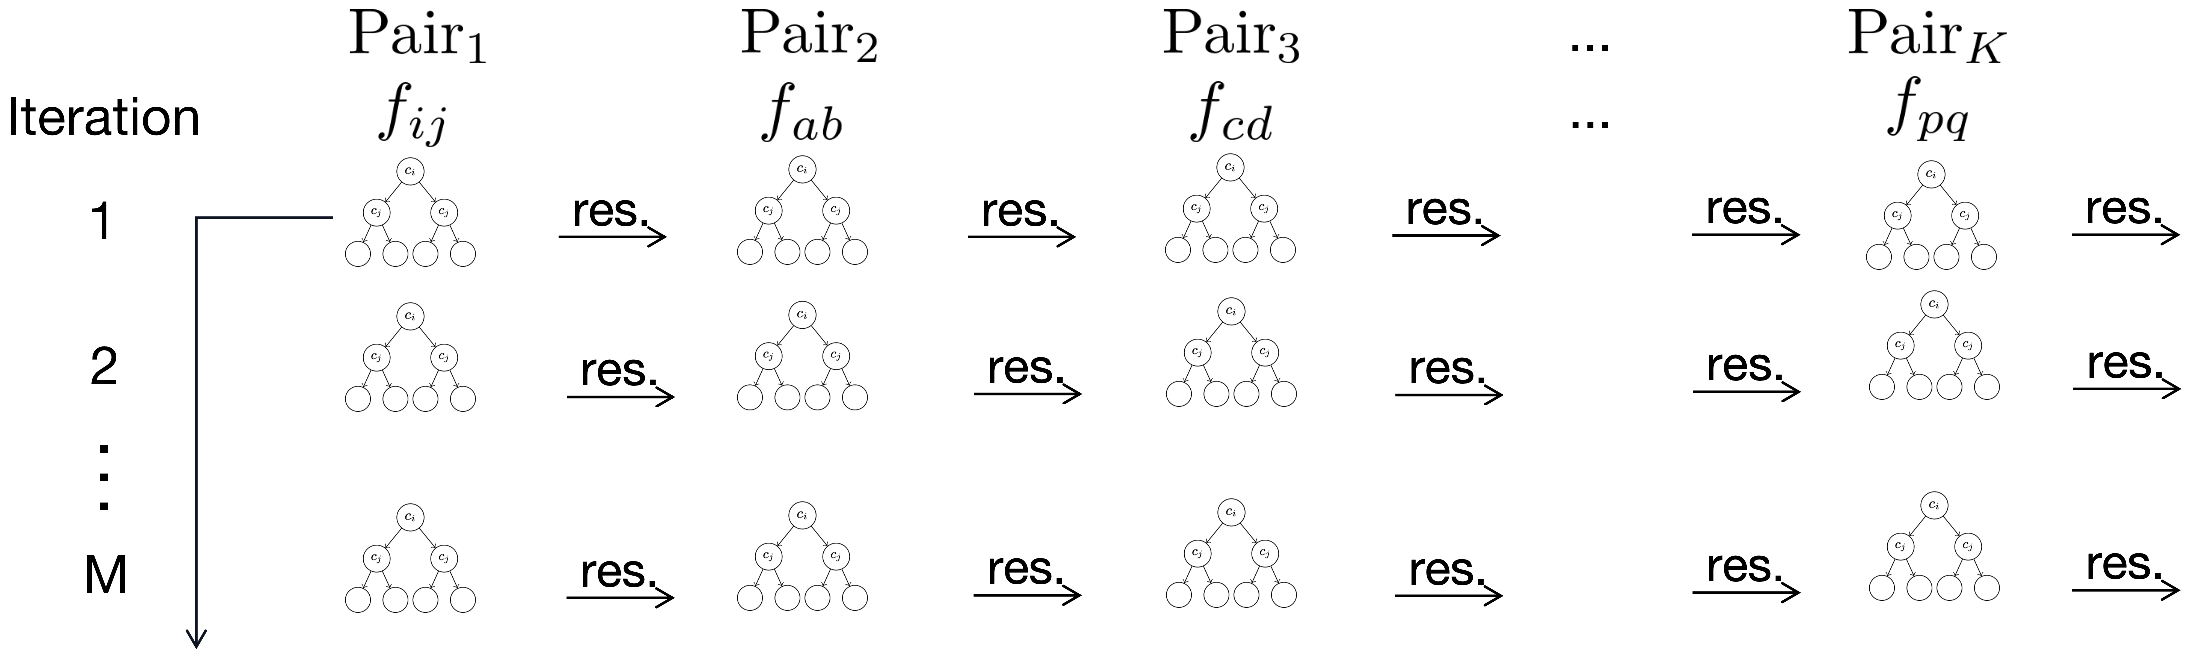
\includegraphics[width=1\linewidth]{figure/GA2M_Step1.png}
%     \label{fig:GA2M_Step1}
% \end{figure}
% \begin{columns}[T, totalwidth=\textwidth]
%     \begin{column}{0.4\textwidth} 
%         \begin{figure}
%             \vspace{-1.35cm} 
%             \hspace{-0.8cm} 
%             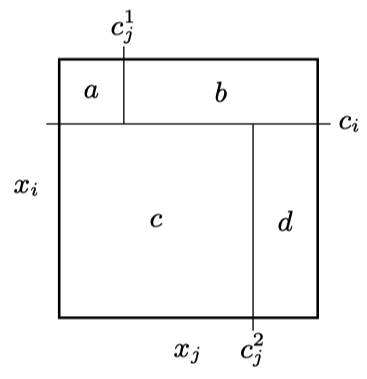
\includegraphics[width=0.8\linewidth]{figure/GA2M_Step0.png}
%             \label{fig:GA2M_predictor}
%         \end{figure}
%     \end{column}
%     \hfill
%     \begin{column}{0.7\textwidth}
%     \begin{itemize}
%       \setlength{\leftskip}{-0.7cm}
%       \vspace{-0.8cm}
%     \item Model each selected pairwise interaction $f_{ij}(x_i, x_j)$ using boosting over residuals
%     \item Replace shallow trees with a tree-like 2D predictor (similar to FAST) but use 3 cuts: 2 axis-aligned ($c_i$, $c_j$) and 1 additional refinement
%     \item Reuse precomputed lookup tables from FAST (sum of targets and counts per region)
%     \item Apply greedy search over cut positions to minimize RSS per boosting step
% \end{itemize}

%         % \begin{itemize}
%         %     \setlength{\leftskip}{-0.7cm}
%         %     \vspace{-0.8cm}
%         %     \item To model the pairwise interactions effectively and efficiently\\
%         %     $\leadsto$Replace the shallow tree ensembles used in Intelligible GAM with a tree-like predictor (similar to FAST)
%         %     \item 3 cuts instead of 2 cuts
%         %     \item Re-use the stored values in the lookup tables for sum of targets and sum of counts from FAST
%         %     \item Greedy search for the best combination of cuts (lowest RSS)
%         % \end{itemize}
%     \end{column}
% \end{columns}

% \end{frame}


\begin{frame}{EBM - Boosting Pairwise Interactions}
%\vspace{-0.2cm}
%\begin{figure}
%    \centering
    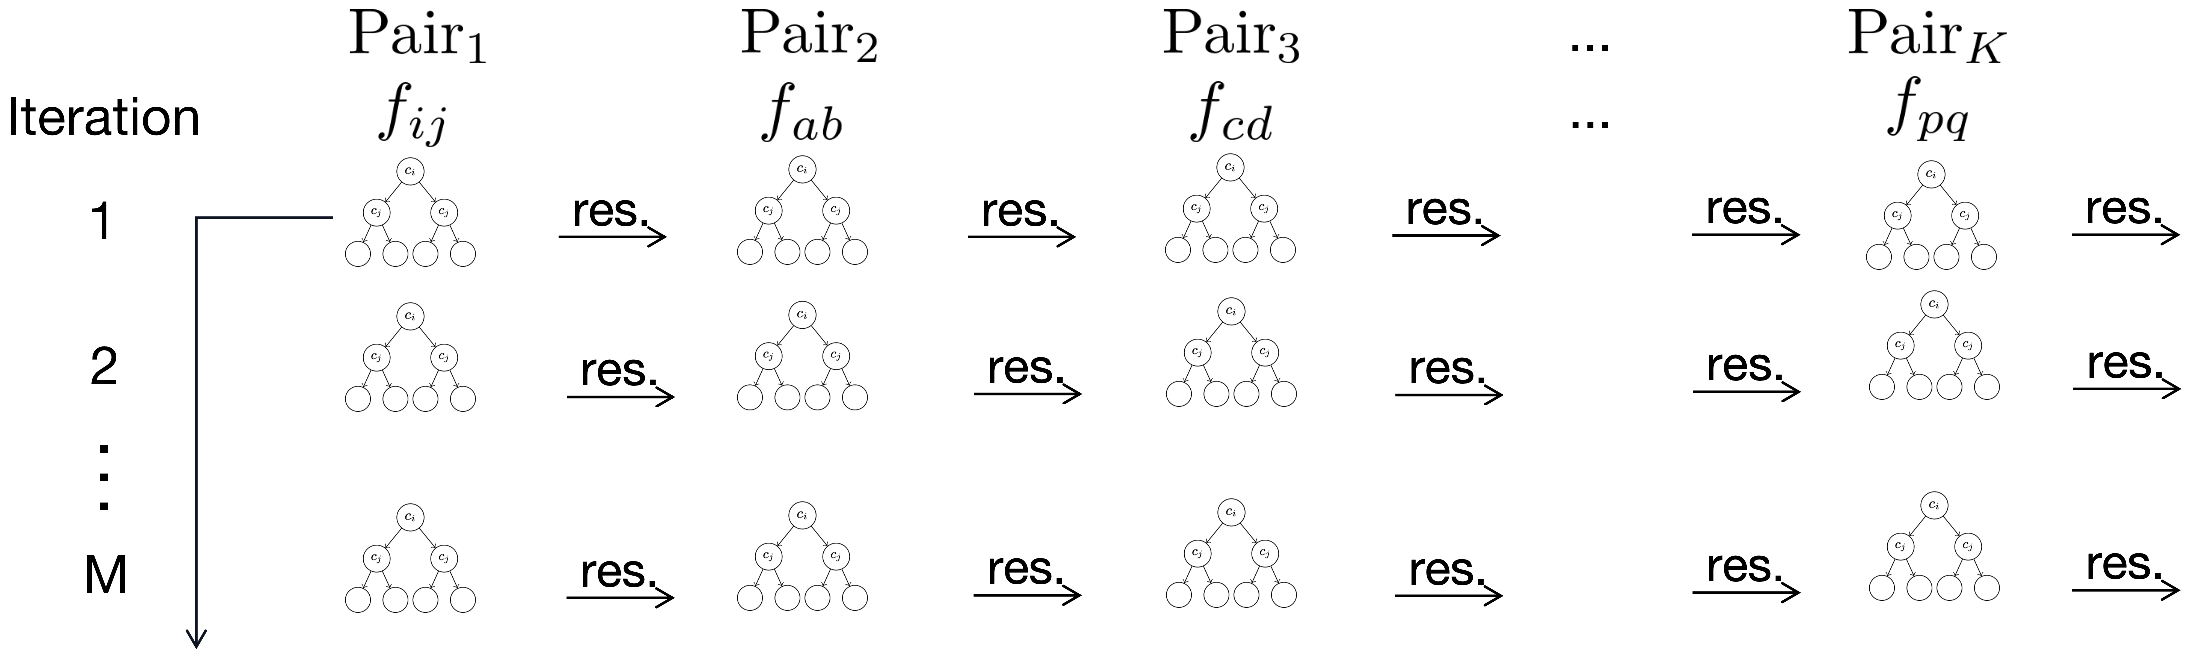
\includegraphics[width=\linewidth]{figure/GA2M_Step1.png}
%\end{figure}

\begin{columns}[c, totalwidth=\textwidth]
    \begin{column}{0.3\textwidth}
        % \vspace{-1.2cm}
        % \hspace{-0.6cm}
        %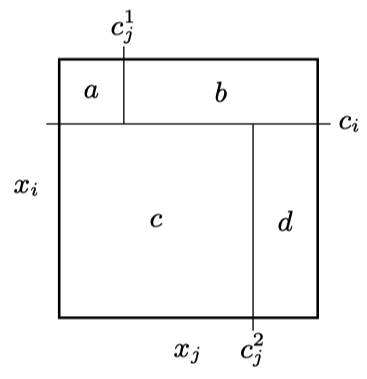
\includegraphics[width=\linewidth]{figure/GA2M_Step0.png}
\begin{center}
    \centering
\begin{tikzpicture}[scale=0.9]

% Rectangle dimensions
\def\W{3.2}
\def\H{3.2}
\def\cxOne{0.9}
\def\cxTwo{2.3}
\def\cy{2.2}

% Outer box
\draw[thick] (0,0) rectangle (\W,\H);

% Internal cuts
\draw[thick] (\cxOne,\cy) -- (\cxOne,\H);
\draw[thick] (\cxTwo,0) -- (\cxTwo,\cy);
\draw[thick] (0,\cy) -- (\W,\cy);

% Region labels
\node at (0.45,2.75) {$\hat{y}_A$};
\node at (1.6,2.75) {$\hat{y}_B$};
\node at (1.1,1.1) {$\hat{y}_C$};
\node at (2.75,1.1) {$\hat{y}_D$};

% Axes and cut labels
\node at (-0.2,\H/2) {$x_i$};
\node at (\W/2,-0.3) {$x_j$};

\node at (-0.3,\cy) {$c_i$};
\node at (\cxOne,3.4) {$c_{j_1}$};
\node at (\cxTwo,-0.3) {$c_{j_2}$};

\end{tikzpicture}

\end{center}
    \end{column}
    
    \begin{column}{0.7\textwidth}
       % \vspace{-0.6cm}
        \begin{itemize}
            \item \textbf{Goal:} Fit each selected interaction $f_{ij}(x_i, x_j)$ on residuals from main effects
            \item Use tree-like predictor, inspired by FAST
            %\item \textbf{Cuts:} 
            \begin{itemize}
                \item Use two axis-aligned cuts $(c_i, c_j)$ 
                \item Plus one refinement cut to increase flexibility while keeping interpretability
            \end{itemize}
            \item Reuse region-wise sums from FAST lookup tables
            \item Greedy search for cut config minimizing RSS
        \end{itemize}
    \end{column}
\end{columns}
\end{frame}


% \begin{frame}{Accurate GAM - Prediction}
% \begin{itemize}
%     \item Output: $M$ predictors which were only trained on $\text{Pair}_1$ \\
%     \qquad\;\; + $M$ predictors which were only trained on $\text{Pair}_2$ \\
%     \qquad\;\; $\cdots$ \\
%     \qquad\;\; + $M$ predictors which were only trained on $\text{Pair}_K$
%     \item Summarize the weighted predictions of $M$ models in a 3D heatmap
%     \item The dimension of color represents the contribution of pairwise feature values to the prediction
%     \item Generate a 3D heatmap for each pair of features
% \end{itemize}

% \begin{figure}    
%     \includegraphics[width=0.4\linewidth]
%     {figure/3D Heatmap.png}
%     \label{fig:3D Heatmap}
% \end{figure}

% \end{frame}

% \begin{frame}{GA2M - Prediction with Pairwise Interactions}
% \begin{itemize}
%     \item Output: $M$ predictors for each of the $K$ selected pairwise interactions $f_{ij}(x_i, x_j)$
%     \item Each $f_{ij}$ is visualized as a 2D heatmap over feature pairs
%     \item Color encodes the contribution of feature value combinations to the final prediction
%     \item Summarize the ensemble of $M$ predictors per pair into a single interpretable surface
% \end{itemize}

% \vspace{0.3cm}
% \centering
% 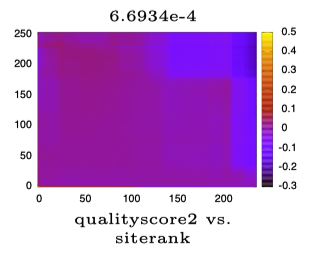
\includegraphics[width=0.42\linewidth]{figure/3D Heatmap.png}
% \end{frame}

\begin{frame}{EBM - Prediction with Pairwise Interactions}
\begin{itemize}
    \item Each selected pair $(x_i, x_j)$ is modeled by $M$ boosted predictors trained on their residual interaction
    \item These are aggregated into a single bivariate function $f_{ij}(x_i, x_j)$
    \item The function is visualized as a 2D heatmap: 
    \begin{itemize}
        \item Axes: feature values of $x_i$ and $x_j$
        \item Color: contribution to the final prediction
        \item Preserves human interpretability 
    \end{itemize}
    \item One heatmap is generated per selected pairwise interaction
\end{itemize}

\vspace{0.3cm}
\centering
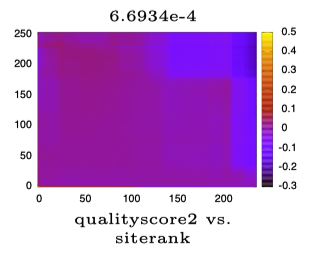
\includegraphics[width=0.42\linewidth]{figure/3D Heatmap.png}
\end{frame}


\begin{frame}{EBM - Final Model Structure}

\begin{itemize}
    \item \textbf{Main effects:} One shape function $f_j(x_j)$ per feature \\(visualized as 1D plots)
    \item \textbf{Pairwise interactions:} Selected functions $f_{ij}(x_i, x_j)$ added for top $K$ pairs (visualized as 2D heatmaps)
    \item \textbf{Prediction:} Additive sum of all univariate and selected bivariate contributions
\end{itemize}

\vspace{0.3cm}
\centering
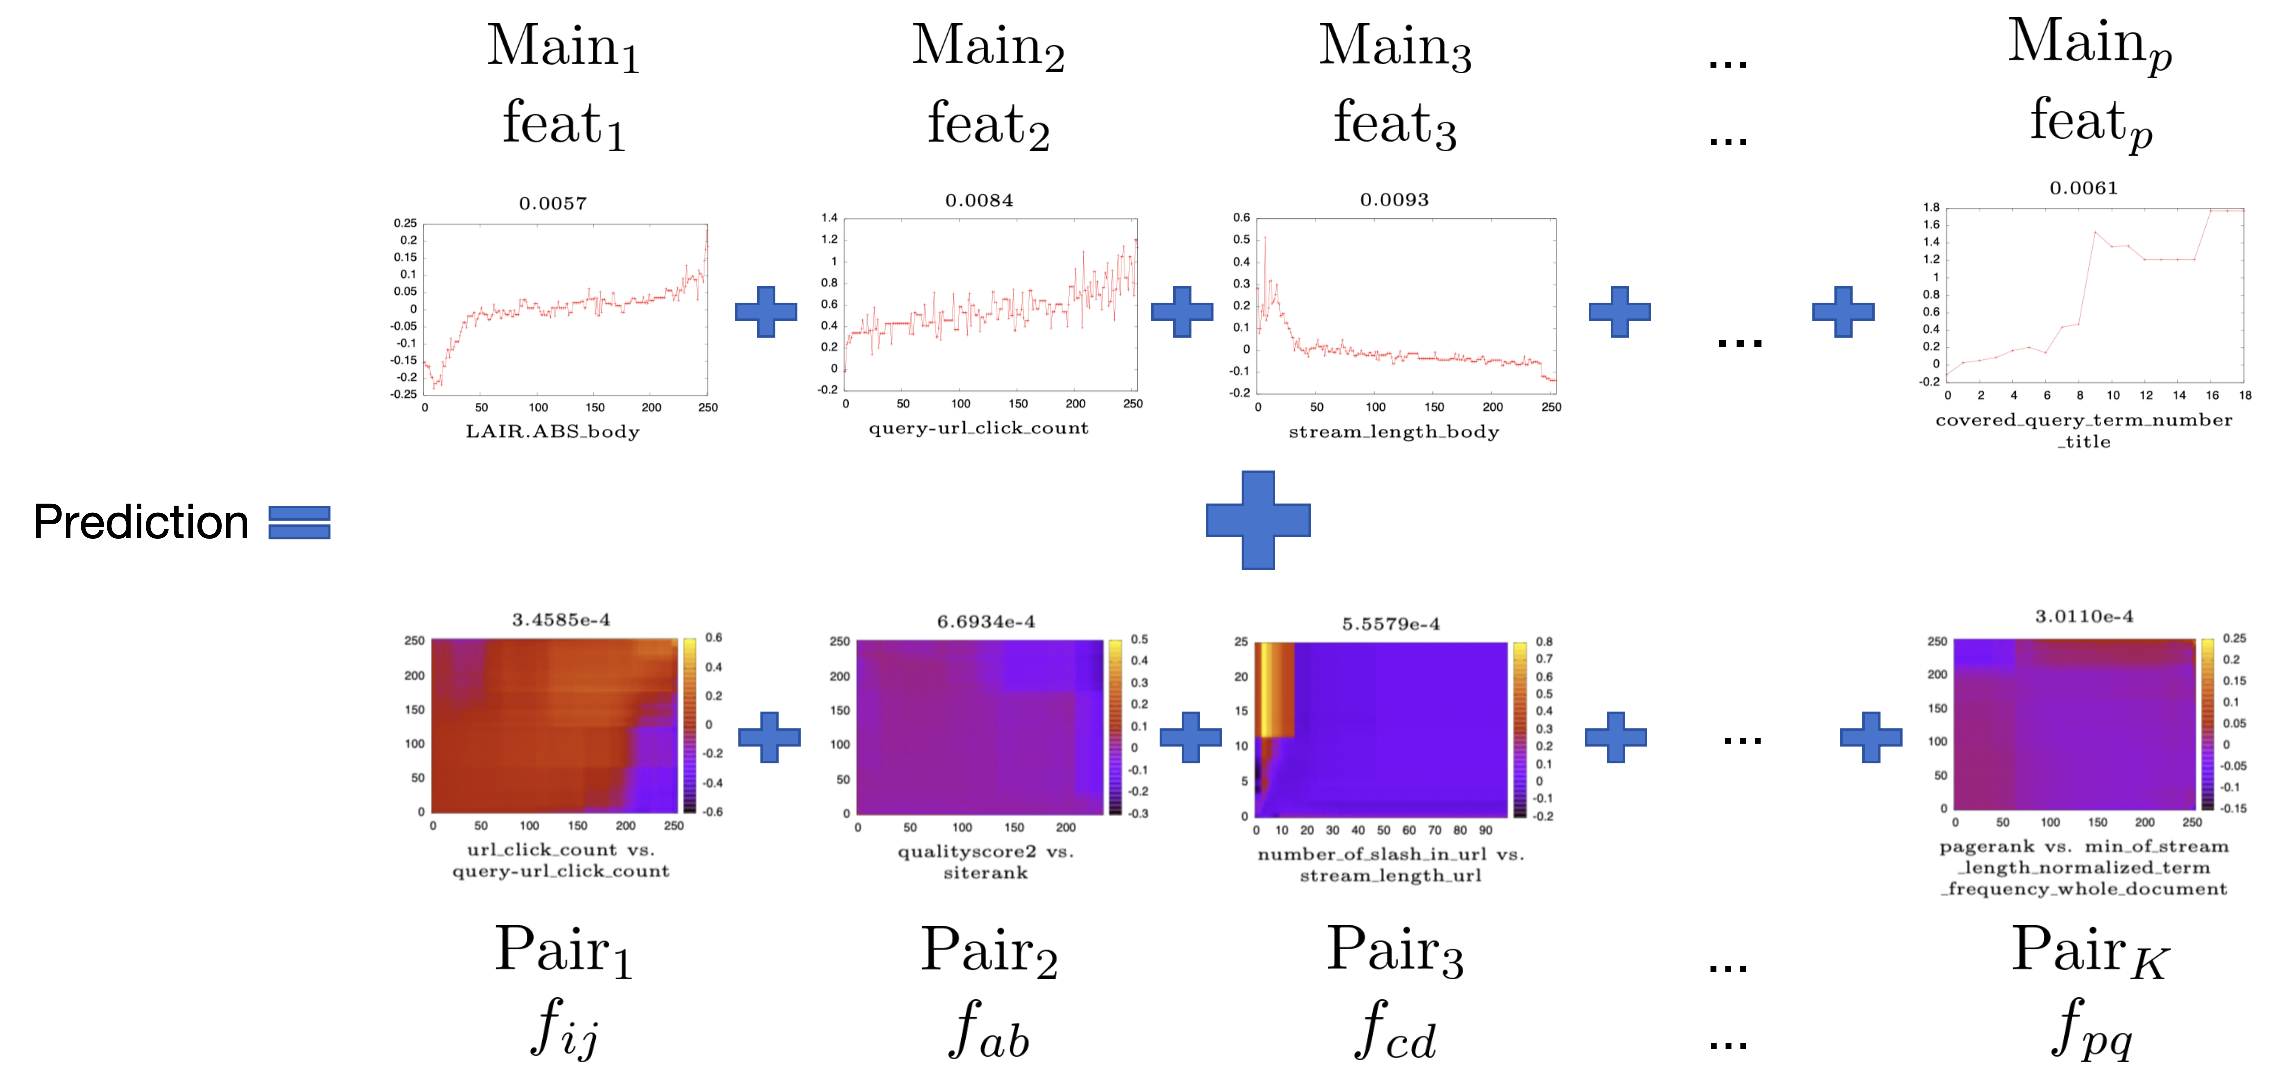
\includegraphics[width=\linewidth]{figure/final_ebm.png}

\end{frame}



% % ---------- SLIDE 1: headline comparison ---------------------------
% \begin{frame}{EBM \textit{vs.} Model-based Boosting}
% \small
% \setlength{\tabcolsep}{5pt}
% \begin{tabular}{@{}p{2.5cm}p{4.5cm}p{4.5cm}@{}}
% \toprule
% \textbf{Aspect} &
% \textbf{EBM \phantom{XXXXXXXXX} % OLD
%\citebutton{Lou et al. 2012}{https://www.cs.cornell.edu/~yinlou/papers/lou-kdd12.pdf}
% new
% \furtherreading{LOU2012} % OLD
%\citebutton{Lou et al. 2013}{https://www.cs.cornell.edu/~yinlou/papers/lou-kdd13.pdf}
% new
% \furtherreading{LOU2013}} &
% \textbf{Model-based Boosting \phantom{XXXX} 
% % OLD
%\citebutton{Buhlmann, 2003}{https://doi.org/10.1198/016214503000125}
% new
% \furtherreading{Buhlmann_2003} % OLD
%\citebutton{Buhlmann, 2008}{https://arxiv.org/abs/0804.2752}
% new
% \furtherreading{Buhlmann_2008}} \\
% \midrule
% \emph{Base learner} &
% Bagged trees (2-4 leaves), one feature at a time; piece-wise constant shape functions &
% Custom learner per component (linear, spline, tree) \\
% \addlinespace[2pt]\pause
% \emph{Iteration policy} &
% Round-robin cycle over \emph{all} features at every boosting iteration &
% Greedy: update \emph{single} component that most reduces risk \\
% \addlinespace[2pt]\pause
% \emph{Regularisation} &
% $\eta\!\approx\!0.01$;\; high $M$ (5-10k) + early stopping via internal CV on OOB samples;\; bagging lowers variance &
% Shrinkage $\nu\!\in\!(0,1]$;\; early stopping;\; intrinsic variable selection \\
% \addlinespace[2pt]\pause
% \emph{Interactions} &
% FAST ranks and selects top-$K$ interaction pairs, fitted as bivariate trees (GA2M) &
% Only included if user provides explicit interaction terms; no automatic pairwise search\\
% \addlinespace[2pt]\pause
% \emph{Interpretability} &
% 1-D step plots ($f_j$) + selected 2-D heat-maps ($f_{ij}$) &
% Depends on base learner: coefficients, smooth splines, random-effect curves, etc.\\
% \bottomrule
% \end{tabular}
% \end{frame}
%------------- SLIDE 1 -------------------------------------------------
\begin{frame}{EBM \textit{vs.} Model-based Boosting}
\small
\begin{itemize}
  %-- BASE LEARNER -----------------------------------------------------
  \item \textbf{Base learner}
        \begin{itemize}
          \item \textbf{EBM}: bagged 2--4-leaf trees, \emph{one feature} per tree  
                $\Rightarrow$ step-function shape $f_j$  % ASCII arrow macro
                % OLD
%\citebutton{Lou et al.\ 2012}{https://www.cs.cornell.edu/~yinlou/papers/lou-kdd12.pdf}
% new
\furtherreading{LOU2012}
          \item \textbf{MB-boost}: user chooses component-wise learner  
                (linear term, P-spline, tree, random effect, \dots)  
                % OLD
%\citebutton{B\"uhlmann \& Hothorn 2007}{https://doi.org/10.1214/07-STS242}
% new
\furtherreading{BÜHLMANNHOTHORN2007}
        \end{itemize}
\pause
  %-- ITERATION POLICY -------------------------------------------------
  \item \textbf{Iteration policy}
        \begin{itemize}
          \item \textbf{EBM}: round-robin ($\forall j$) each boosting pass; \\tiny
                learning rate $\eta \approx 0.01$.
          \item \textbf{MB-boost}: greedy; update the \emph{single} component that yields the largest loss reduction.
        \end{itemize}
\pause
  %-- REGULARISATION ---------------------------------------------------
  \item \textbf{Regularisation}
        \begin{itemize}
          \item \textbf{EBM}: many iterations $M$ (5--10k);  
                early stopping via \emph{internal} CV on out-of-bag samples;  
                bagging further lowers variance.
          \item \textbf{MB-boost}: shrinkage $\nu \in (0,1]$;  
                early stop by CV/AIC; component selection acts like an
                $L_0/L_1$ penalty $\rightarrow$ sparsity.
        \end{itemize}
\end{itemize}
\end{frame}

%------------- SLIDE 2 -------------------------------------------------
\begin{frame}{EBM \textit{vs.} Model-based Boosting}
\small
\begin{itemize}
  %-- INTERACTIONS -----------------------------------------------------
  \item \textbf{Interactions}
        \begin{itemize}
          \item \textbf{EBM}: FAST ranks and selects top-$K$ interaction pairs, fitted as bivariate trees $\Rightarrow$ GA2M  
                % OLD
%\citebutton{Lou et~al.\ 2013}{https://www.cs.cornell.edu/~yinlou/papers/lou-kdd13.pdf}
% new
\furtherreading{LOU2013}
          \item \textbf{MB-boost}: interactions are modelled only when the
                user supplies dedicated interaction base learners;
                no automatic pairwise search
        \end{itemize}
\pause
  %-- INTERPRETABILITY -------------------------------------------------
  \item \textbf{Interpretability}
        \begin{itemize}
          \item \textbf{EBM}:
          \begin{itemize}
              \item one\;1-D step plot for each $f_{j}$
              \item small number of 2-D heat-maps for selected $f_{ij}$
          \end{itemize} 
          \item \textbf{MB-boost}: depends on selected learner: linear
                coefficients, smooth splines, random-effect curves, etc. %; statistical inference (confidence intervals, $p$-values) available for many bases
        \end{itemize}
\pause
  %-- TAKE-AWAY --------------------------------------------------------
  \item \textbf{Take-away}  
  \begin{itemize}
      \item \emph{EBM} provides fast, interpretable, and interaction-sparse models
      \item \emph{MB-boost} offers flexible stat modeling with built-in variable selection %and formal inference
  \end{itemize}
\end{itemize}
\end{frame}


\endlecture
\end{document}